\chapter{PENGUJIAN DAN ANALISIS}
\label{chap:pengujiananalisis}

% Ubah bagian-bagian berikut dengan isi dari pengujian dan analisis

Penelitian dilakukan dengan melakukan uji dan anaisa dari sistem yang telah dibuat berdasarkan langkah pada metodologi yang telah dilaksanakan. Pengujian ini dilakukan untuk menguji kemampuan sistem yang telah dibuat dalam menjawab permasalahan yang dijadikan acuan pada penelitian ini untuk mendapatkan hasil dari tujuan yang ingin didapat. Skenario pengujian dan pembahasan yang dilakukan pada penelitian ini, antara lain:

\begin{enumerate}[nolistsep]

  \item Pengujian Hasil \emph{Training}, \emph{Validation} dan \emph{Testing} Model

  \item Pengujian Deteksi Langkah 

  \item Pengujian Prediksi Kalori
  
  \item Pengujian Performa Berdasarkan Jarak Kamera
  
  \item Pengujian Performa Berdasarkan Posisi Kamera
  
  \item Pengujian Performa Berdasarkan Intensitas Cahaya
  
  \item Pengujian Sistem secara \emph{Real Time}

\end{enumerate}

\section{Pengujian Hasil \emph{Training}, \emph{Validation} dan \emph{Testing} Model}
\label{sec:PengujianTrainingValidation}

Pengujian pembuatan model berdasarkan hasil \emph{training} dan \emph{validation} dengan menggunakan dataset dengan jumlah keseluruhan yaitu 1731 sampel data. Dengan jumlah sample training sebanyak 1385 dan sampel validation sebanyak 346. Setelah dilakukan proses \emph{training} dan \emph{validation} terhadap dataset yang telah ditentukan oleh sampel data, didapatkan hasil pengujian akurasi dengan tingkat akurasi training sebesar 0,951 dan tingkat akurasi validation sebesar 0,977. Kemudian didapatkan hasil pengujian loss pada training sebesar 0,127 dan loss pada validation sebesar 0,059. Hasil pengujian ditunjukkan pada grafik nilai akurasi dan loss pada proses \emph{training} dan \emph{validation} seperti pada Gambar \ref{fig:HasilTrainingValidation}.

\begin{figure}[H]
  \centering
  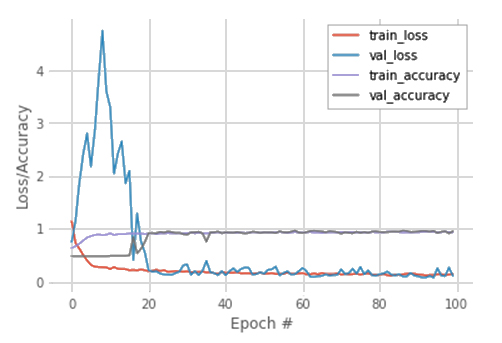
\includegraphics[scale=0.6]{gambar/hasil training dan validation w.jpg}
  \caption{Grafik hasil \emph{training} dan \emph{validation}}
  \label{fig:HasilTrainingValidation}
\end{figure}

Pengujian dilanjutkan dengan melakukan \emph{testing} model dengan menggunakan dataset yang sudah dimiliki dengan jumlah keseluruhan yaitu 347 sampel data. Dataset yang digunakan merupakan dataset yang sudah dilakukan filtrasi yang hanya digunakan pada pengujian \emph{testing} saja. Hasil pengujian \emph{testing} model didapatkan akurasi sebesar 95\% dengan hasil deteksi benar untuk kelas kanan sebanyak 170 sampel 96\% dan kelas kiri sebanyak 161 sampel 95\%. Pengujian ditunjukkan dengan confusion matrix pada Gambar \ref{fig:HasilTesting} dan Tabel \ref{tb:ClassificationReport} merupakan classification report dari hasil pengujian yang telah dilakukan pada pengujian \emph{testing} model penelitian ini.

\begin{figure}[H]
  \centering
  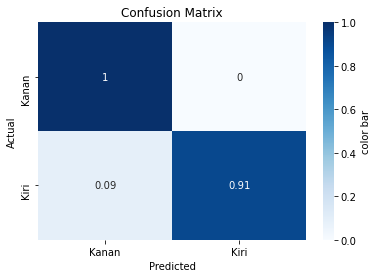
\includegraphics[scale=1]{gambar/cm normalized.png}
  \caption{\emph{Confusion Matrix} hasil \emph{testing} model}
  \label{fig:HasilTesting}
\end{figure}

\begin{longtable}{|c|c|c|c|c|}
  \caption{\emph{Classification Report} hasil pengujian \emph{testing} model}
  \label{tb:ClassificationReport}                                   \\
  \hline
  \rowcolor[HTML]{C0C0C0}
   & \textbf{Precision} & \textbf{Recall} & \textbf{F1-Score} & \textbf{Support} \\
  \hline
  kanan     & 0,91    & 1,00    & 0,96    & 170         \\
  \hline
  kiri      & 1,00    & 0,91    & 0,95    & 177           \\
  \hline
  Accuracy  &         &         & 0,95    & 347            \\
  \hline
\end{longtable}

Model yang digunakan pada penelitiian ini terdapat dua macam yang akan digunakan pada proses klasifikasi langkah. Pada model yang telah dibuat dan telah dianalisa sebelumnya merupakan model yang digunakan pada sebagian besar pengujian pada penelitian ini. Posisi yang diambil untuk melakukan pembuatan model dengan posisi untuk melakukan klasifikasi dari arah samping objek yang akan dilakukan deteksi. Pada pengujian terdapat pengujian yang akan dilakukan dari posisi belakang objek. Dengan menggunakan posisi tersebut maka dibutuhkan model klasifikasi yang berbeda melihat dari proses estimasi pose dan data yang didapat memiliki karakteristik yang berbeda pada pengujian ini. 

Pembuatan model kedua dilakukan kembali proses estimasi pose untuk mendapatkan dataset yang kemudian dilakukan pembuatan model. Hasil estimasi dilakukan proses ekstrak fitur dan proses pelabelan objek. Dataset yang dibuat memiliki jumlah kelas yang sama yaitu terdapat dua kelas kanan dan kelas kiri. Hasil ekstrak fitur dan dilakukannya proses \emph{preprocessing} menghasilkan gambar dataset kelas kanan dan kelas kiri. Gambar \ref{fig:KelasBelakangKanan} menunjukkan gambar dataset kelas kanan dan Gambar \ref{fig:KelasBelakangKiri} menunjukkan gambar dataset kelas kiri.

\begin{figure}[H]
  \centering
  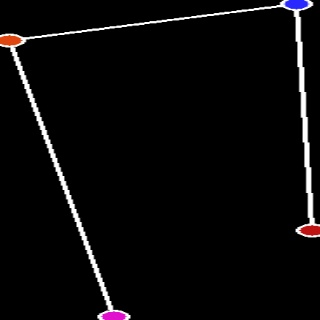
\includegraphics[scale=0.45]{gambar/dataset belakang kanan.jpg}
  \caption{Hasil \emph{preprocessing} untuk model kedua kelas kanan}
  \label{fig:KelasBelakangKanan}
\end{figure}

\begin{figure}[H]
  \centering
  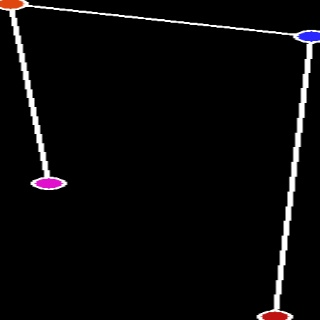
\includegraphics[scale=0.45]{gambar/dataset belakang kiri.jpg}
  \caption{Hasil \emph{preprocessing} untuk model kedua kelas kiri}
  \label{fig:KelasBelakangKiri}
\end{figure}

Hasil gambar digunakan pada dataset yang akan dilakukan pelabelan objek untuk dapat memberikan informasi nama kelas dari objek yang akan dideteksi pada model ini. Label yang diberikan pada dataset sesuai dengan kelas yaitu label kanan dan label kiri. Dari setiap gambar yang telah dilakukan ekstraksi fitur dilakukan pemberian label sesuai kelas yang digunakan Hasil pelabelan objek gambar tersebut ditunjukkan pada Tabel 

\begin{longtable}{|c|c|}
  \caption{Hasil anotasi dari pelabelan objek model kedua}
  \label{tb:HasilAnotasi}  \\
  \hline
  \rowcolor[HTML]{C0C0C0}
  \textbf{Kelas} & \textbf{Jumlah Anotasi}  \\
  \hline
  Kanan           & 896    \\
  \hline
  Kiri            & 860    \\
  \hline
  \textbf{Total}  & \textbf{1.756}  \\
  \hline
\end{longtable}

Dataset yang telah dilakukan anotasi untuk pelabelan objek dilakukan proses pembuatan model klasifikasi. Dengan menggunakan arsitetkur yang sama dilakukan proses \emph{training} untuk mendapatkan hasil \emph{training} dan \emph{validation} yang kemudian dilakukan \emph{testing} model yang telah dibuat terhadap dataset. Pengujian pembuatan model berdasarkan hasil \emph{training} dan \emph{validation} dengan menggunakan dataset dengan jumlah keseluruhan yaitu 1756 sampel data. Dengan jumlah sample training sebanyak 1405 dan sampel validation sebanyak 317. Setelah dilakukan proses \emph{training} dan \emph{validation} terhadap dataset yang telah ditentukan oleh sampel data, didapatkan hasil pengujian akurasi dengan tingkat akurasi training sebesar 0,959 dan tingkat akurasi validation sebesar 0,972. Kemudian didapatkan hasil pengujian loss pada training sebesar 0,107 dan loss pada validation sebesar 0,053. Hasil pengujian ditunjukkan pada grafik nilai akurasi dan loss pada proses \emph{training} dan \emph{validation} seperti pada Gambar \ref{fig:HasilTrainingValidationModel2}.

\begin{figure}[H]
  \centering
  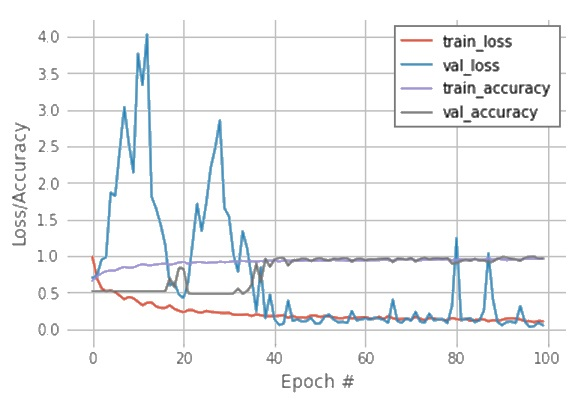
\includegraphics[scale=0.75]{gambar/belakang w.jpg}
  \caption{Grafik hasil \emph{training} dan \emph{validation} model kedua}
  \label{fig:HasilTrainingValidationModel2}
\end{figure}

Pengujian dilanjutkan dengan melakukan \emph{testing} model dengan menggunakan dataset yang sudah dimiliki dengan jumlah keseluruhan yaitu 317 sampel data. Dataset yang digunakan merupakan dataset yang sudah dilakukan filtrasi yang hanya digunakan pada pengujian \emph{testing} saja. Hasil pengujian \emph{testing} model didapatkan akurasi sebesar 90\% dengan hasil deteksi benar untuk kelas kanan sebanyak 158 sampel 90\% dan kelas kiri sebanyak 182 sampel 91\%. Pengujian ditunjukkan dengan confusion matrix pada Gambar \ref{fig:HasilTestingModel2} dan Tabel \ref{tb:ClassificationReportModel2} merupakan classification report dari hasil pengujian yang telah dilakukan pada pengujian \emph{testing} model penelitian ini.

\begin{figure}[H]
  \centering
  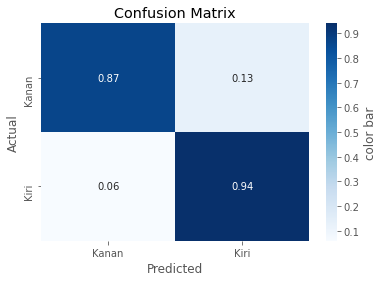
\includegraphics[scale=1]{gambar/cm model belakang.png}
  \caption{\emph{Confusion Matrix} hasil \emph{testing} model kedua}
  \label{fig:HasilTestingModel2}
\end{figure}

\begin{longtable}{|c|c|c|c|c|}
  \caption{\emph{Classification Report} hasil pengujian \emph{testing} model kedua}
  \label{tb:ClassificationReportModel2}                                   \\
  \hline
  \rowcolor[HTML]{C0C0C0}
   & \textbf{Precision} & \textbf{Recall} & \textbf{F1-Score} & \textbf{Support} \\
  \hline
  kanan     & 0,94    & 0,87    & 0,90    & 179         \\
  \hline
  kiri      & 0,87    & 0,94    & 0,91    & 172           \\
  \hline
  Accuracy  &         &         & 0,90    & 351            \\
  \hline
\end{longtable}

\section{Pengujian Hasil Deteksi}
\label{sec:PengujianDeteksi}

Proses deteksi yang dilakukan dengan menggunakan model yang telah dibuat dilakukan pengujian dari hasil yang didapat dari hasil deteksi dengan perhitungan yang sebenarnya. Pengujian dilakukan dengan membuat data sebenarnya dengan melakukan perhitungan langkah dari akuisisi maupun data video yang digunakan dalam percobaan dan dibandingkan dengan hasil perhitungan langkah dari hasil deteksi. Tabel \ref{tb:PengujianDeteksi} menunjukkan hasil perhitungan data sebenarnya dengan data hasil deteksi terhadap langkah pada data video. 

\begin{longtable}{|c|c|c|}
  \caption{Pengujian Hasil Deteksi}
  \label{tb:PengujianDeteksi}                                   \\
  \hline
  \rowcolor[HTML]{C0C0C0}
  \textbf{Percobaan} & \textbf{Langkah} & \textbf{Deteksi Langkah} \\
  \hline
  1   & 241   & 328    \\
  \hline
  2   & 169   & 170    \\
  \hline
  3   & 302   & 302    \\
  \hline
  4   & 246   & 248    \\
  \hline
  5   & 321   & 322    \\
  \hline
  6   & 220   & 218    \\
  \hline
  7   & 274   & 274    \\
  \hline
  8   & 260   & 256    \\
  \hline
  9   & 276   & 260    \\
  \hline
  10   & 321   & 334    \\
  \hline
  11   & 309   & 314    \\
  \hline
  12   & 317   & 276    \\
  \hline
  13   & 276   & 244    \\
  \hline
  14   & 259   & 260    \\
  \hline
  15   & 292   & 231    \\
  \hline
  16   & 117   & 116    \\
  \hline
  17   & 141   & 144    \\
  \hline
\end{longtable}

Pengujian dilakukan setelah didapatkan data hasil deteksi yang telah didapat dan juga data sebenarnya berdasarkan hasil perhitungan yang dilakukan terhadap data video. Setiap percobaan dilakukan analisa terkait perbandingan hasil yang didapat antara data hasil deteksi dan data perhitungan sebenarnya. Perbandingan dilakukan dengan mencari nilai eror dari hasil perbedaan yang didapat dari setiap data percobaan untuk kemudian ditentukan dan dikalkulasikan dalam hasil akurasi dan error yang didapat dari analisa tersebut. Hasil analisa yang didapat dengan melakukan analisa pengujian hasil deteksi didapatkan hasil akurasi rata-rata sebesar 96,14\% dengan hasil eror rata-rata sebesar 3,86\%. Tabel \ref{tb:AnalisaDeteksi} menunjukkan hasil analisa dari setiap percobaan yang dilakukan analisa pengujian.

\begin{longtable}{|c|c|c|c|c|c|}
  \caption{Analisa Pengujian Hasil Deteksi}
  \label{tb:AnalisaDeteksi}                                   \\
  \hline
  \rowcolor[HTML]{C0C0C0}
  \textbf{Percobaan} & \textbf{Langkah} & \textbf{Deteksi Langkah} & \textbf{Eror} & \textbf{Eror\%} & \textbf{Akurasi\%} \\
  \hline
  1   & 241   & 238   & 3    & 1,24\%    & 98,76\%   \\
  \hline
  2   & 169   & 170   & 1    & 0,59\%    & 99,41\%   \\
  \hline
  3   & 302   & 302   & 0    & 0\%       & 100\%     \\
  \hline
  4   & 246   & 248   & 2    & 0,81\%    & 99,19\%   \\
  \hline
  5   & 321   & 322   & 1    & 0,31\%    & 99,69\%   \\
  \hline
  6   & 220   & 218   & 2    & 0,91\%    & 99,09\%   \\
  \hline
  7   & 274   & 274   & 0    & 0\%       & 100\%   \\
  \hline
  8   & 260   & 256   & 4    & 1,54\%    & 98,46\%   \\
  \hline
  9   & 276   & 260   & 16   & 5,80\%    & 94,20\%   \\
  \hline
  10   & 321   & 334  & 13   & 4,05\%    & 95,95\%   \\
  \hline
  11   & 309   & 314  & 5    & 1,62\%    & 98,38\%   \\
  \hline
  12   & 317   & 276  & 41   & 12,93\%   & 87,07\%   \\
  \hline
  13   & 276   & 244  & 32   & 11,59\%   & 88,41\%   \\
  \hline
  14   & 259   & 260  & 1    & 0,39\%    & 99,61\%   \\
  \hline
  15   & 292   & 231  & 61   & 20,89\%   & 79,11\%   \\
  \hline
  16   & 117   & 116  & 1    & 0,85\%    & 99,15\%   \\
  \hline
  17   & 141   & 144  & 3    & 2,13\%    & 97,87\%   \\
  \hline

  \multicolumn{4}{|c|}{\textbf{Rata-rata}} & 3,86\% & 96,14\% \\
  \hline
\end{longtable}


\section{Pengujian Prediksi Kalori}
\label{sec:PengujianPrediksi}

Pengujian pada prediksi jumlah kalori yang terbakar dilakukan setelah melakukan pengujian pada model deteksi yang telah dilakukan. Prediksi dilakukan dengan dua metode, yaitu regresi linear dan perhitungan rumus. Dengan menggunakan dataset berupa citra video yang akan digunakan untuk melakukan prediksi kalori sebanyak 17 sampel video sehingga terdapat 17 percobaan yang dilakukan. Video pengujian menggunakan variasi kecepatan dan hasil kalori yang didapatkan. Variasi kecepatan yang digunakan adalah 3 km/jam, 6 km/jam, 8 km/jam, 9 km/jam dan 12 km/jam. Kemudian variasi hasil kalori yang didapatkan adalah 5, 10 dan 20 kcal. 

\subsection{Prediksi dengan Regresi Linear}
\label{subsec:PengujianPrediksiRegresi}

Pada pengujian dengan regresi linear dengan melakukan proses deteksi dan menggunakan model regresi linear dalam melakukan proses prediksi kalori didapatkan beberapa data pendukung dalam hasil deteksi dan data dari hasil regresi prediksi kalori. Data video yang digunakan sebagai pengujian dilakukan proses deteksi sehingga mendapatkan beberapa data yang akan digunakan dalam proses prediksi kalori. Data deteksi langkah merupakan data hasil deteksi langkah yang didapat dari sistem terhadap data video. Data waktu didapat dari hasil waktu tempuh yang dilakukan selama melakukan proses deteksi pada data video. Dengan data yang didapat dari hasil deteksi berupa langkah dan waktu akan dilakukan akumulasi untuk mendapatkan data jarak dan prediksi kalori dengan regresi linear berdasarkan model yang sudah dibuat sehingga mendapatkan data prediksi kalori. Tabel \ref{tb:PengujianPrediksiRegresi} menunjukkan hasil deteksi dan hasil prediksi kalori dengan menggunakan regresi linear.

\begin{longtable}{|c|c|c|c|c|}
  \caption{Pengujian Prediksi dengan Regresi Linear}
  \label{tb:PengujianPrediksiRegresi}                                   \\
  \hline
  \rowcolor[HTML]{C0C0C0}
  \textbf{Percobaan} & \textbf{Deteksi Langkah} & \textbf{Jarak} & \textbf{Waktu} & \textbf{Prediksi Kalori} \\
  \hline
  1   & 238   & 167,181    & 2:50    & 11,652  \\
  \hline
  2   & 170   & 118,437    & 1:35    & 8,245   \\
  \hline
  3   & 302   & 293,143    & 2:02    & 20,534  \\
  \hline
  4   & 248   & 284,417    & 1:41    & 19,927  \\
  \hline
  5   & 322   & 287,577    & 2:03    & 20,14   \\
  \hline
  6   & 218   & 286,18     & 1:21    & 20,056  \\
  \hline
  7   & 274   & 175,936    & 2:49    & 12,267  \\
  \hline
  8   & 256   & 177,101    & 2:49    & 12,349  \\
  \hline
  9   & 260   & 177,780    & 2:49    & 12,397  \\
  \hline
  10   & 334   & 505,568   & 2:01    & 35,488  \\
  \hline
  11   & 314   & 312,691   & 2:02    & 21,909  \\
  \hline
  12   & 276   & 155,812   & 2:02    & 10,865  \\
  \hline
  13   & 244   & 216,140   & 1:39    & 15,119  \\
  \hline
  14   & 260   & 280,461   & 1:40    & 19,647  \\
  \hline
  15   & 231   & 150,241   & 1:45    & 10,478  \\
  \hline
  16   & 116   & 78,449    & 1:08    & 5,435  \\
  \hline
  17   & 144   & 142,144   & 0:59    & 9,922  \\
  \hline
\end{longtable}

Pada pengujian prediksi kalori dilakukan berdasarkan hasil deteksi yang didapat. Analisa pengujian hasil prediksi kalori dilakukan dengan melakukan perbandingan data prediksi kalori dari sistem yang digunakan dengan data kalori treadmill sebagai data sebenarnya atau data \emph{actual score}. Perbandingan hasil prediksi kalori dengan kalori treadmill didapatkan data eror yang kemudian dilakukan perhitungan persentase berdasarkan data sebenarnya pada data kalori treadmill. Proses analisa pengujian dilakukan terhadap seluruh data video pada data percobaan. Hasil analisa yang didapat dengan melakukan analisa pengujian prediksi kalori didapatkan hasil akurasi rata-rata sebesar 80,93\% dengan hasil eror rata-rata sebesar 19,07\%. Tabel \ref{tb:AnalisaPrediksiRegresi} menunjukkan hasil analisa pengujian dari setiap percobaan yang dilakukan analisa prediksi kalori dengan regresi linear.

\begin{longtable}{|c|c|c|c|c|c|}
  \caption{Analisa Pengujian Prediksi dengan Regresi Linear}
  \label{tb:AnalisaPrediksiRegresi}                                   \\
  \hline
  \rowcolor[HTML]{C0C0C0}
  \textbf{Percobaan} & \textbf{Kalori Treadmill} & \textbf{Prediksi Kalori} & \textbf{Eror} & \textbf{Eror\%} & \textbf{Akurasi\%} \\
  \hline
  1   & 10   & 11,652   & 1,652    & 16,52\%     & 83,48\%   \\
  \hline
  2   & 10   & 8,245    & 1,755    & 17,55\%     & 82,45\%   \\
  \hline
  3   & 20   & 20,534   & 0,534    & 2,67\%      & 97,33\%   \\
  \hline
  4   & 20   & 19,927   & 0,073    & 0,365\%     & 99,635\%  \\
  \hline
  5   & 20   & 20,14    & 0,14     & 0,7\%       & 99,3\%    \\
  \hline
  6   & 20   & 20,056   & 0,056    & 0,28\%      & 99,72\%   \\
  \hline
  7   & 10   & 12,267   & 2,267    & 22,67\%     & 77,33\%   \\
  \hline
  8   & 10   & 12,349   & 2,349    & 23,49\%     & 76,51\%   \\
  \hline
  9   & 10   & 12,397   & 2,397    & 23,97\%     & 76,03\%   \\
  \hline
  10   & 20   & 35,488   & 15,488   & 77,44\%     & 22,56\%   \\
  \hline
  11   & 20   & 21,909   & 1,909    & 9,55\%      & 90,45\%   \\
  \hline
  12   & 20   & 10,865   & 9,135    & 45,67\%     & 54,33\%   \\
  \hline
  13   & 20   & 15,119   & 4,881    & 24,41\%     & 75,59\%   \\
  \hline
  14   & 20   & 19,647   & 0,353    & 1,77\%      & 98,23\%   \\
  \hline
  15   & 20   & 10,478   & 9,522    & 47,61\%     & 52,39\%   \\
  \hline
  16   & 5   & 5,435    & 0,435     & 8,70\%      & 91,03\%   \\
  \hline
  17   & 10   & 9,922    & 0,078    & 0,78\%      & 99,22\%   \\
  \hline

  \multicolumn{4}{|c|}{\textbf{Rata-rata}} & 19,07\% & 80,93\% \\
  \hline
\end{longtable}

\subsection{Prediksi dengan Perhitungan Rumus}
\label{subsec:PengujianPrediksiPerhitungan}

Pada pengujian dengan perhitungan rumus berdasarkan MET dilakukan dengan proses deteksi dan menggunakan perhitungan rumus untuk menghitung prediksi kalori yang terbakar didapatkan data pendukung dalam hasil deteksi dan data dari hasil perhitungan prediksi kalori. Data video yang digunakan sebagai pengujian dilakukan proses deteksi sehingga mendapatkan beberapa data yang akan digunakan dalam proses prediksi kalori. Data deteksi kecepatan merupakan data hasil deteksi yang sudah diproses untuk bisa menentukan kecepatan yang dilakukan dalam proses deteksi. Data MET merupakan data prediksi MET berdasarkan kecepatan yang ditempuh dengan menggunakan model regresi MET. Data waktu didapat dari hasil waktu tempuh yang dilakukan selama proses deteksi pada data video. Dengan data yang didapat dari hasil deteksi dan proses yang dilakukan dapat dilakukan perhitungan rumus dengan menggunakan data MET dan waktu untuk menghitung dan mendapatkan data prediksi kalori dengan rumus yang digunakan. Tabel \ref{tb:PengujianPrediksiPerhitungan} menunjukkan hasil deteksi dan hasil prediksi kalori dengan menggunakan perhitungan rumus.

\begin{longtable}{|c|c|c|c|c|}
  \caption{Pengujian Prediksi dengan Perhitungan Rumus}
  \label{tb:PengujianPrediksiPerhitungan}                                   \\
  \hline
  \rowcolor[HTML]{C0C0C0}
  \textbf{Percobaan} & \textbf{Deteksi Kecepatan} & \textbf{MET} & \textbf{Waktu} & \textbf{Kalori} \\
  \hline
  1   & 3,626   & 2,003    & 2:50    & 6,788   \\
  \hline
  2   & 5,016   & 2,733    & 1:35    & 4.744   \\
  \hline
  3   & 8,943   & 9,323    & 2:02    & 22.462  \\
  \hline
  4   & 10,893  & 10,721   & 1:41    & 20.575  \\
  \hline
  5   & 8,151   & 8,533    & 2:03    & 22.126  \\
  \hline
  6   & 13,041  & 11,985   & 1:21    & 19.331  \\
  \hline
  7   & 3,572   & 2,178    & 2:49    & 6,979  \\
  \hline
  8   & 3,862   & 1,029    & 2:49    & 3,296  \\
  \hline
  9   & 3,820   & 1,192    & 2:49    & 3,819  \\
  \hline
  10   & 15,114   & 13,453   & 2:01    & 30,862  \\
  \hline
  11   & 9,311   & 9,609   & 2:02    & 22,224  \\
  \hline
  12   & 4,557   & 1,396   & 2:02    & 3,228  \\
  \hline
  13   & 8,105   & 8,471   & 1:39    & 15,900  \\
  \hline
  14   & 10,234   & 10,270   & 1:40    & 19,470  \\
  \hline
  15   & 6,326   & 5,832   & 1:45    & 11,057  \\
  \hline
  16   & 4,284   & 0,499    & 1:08    & 0,643  \\
  \hline
  17   & 8,966   & 9,322   & 0:59    & 10,427  \\
  \hline
\end{longtable}

Pada pengujian prediksi kalori dilakukan berdasarkan hasil deteksi yang didapat. Analisa pengujian hasil prediksi kalori dilakukan dengan melakukan perbandingan data prediksi kalori dari sistem yang digunakan dengan data kalori treadmill sebagai data sebenarnya atau data \emph{actual score}. Perbandingan hasil prediksi kalori dengan kalori treadmill didapatkan data eror yang kemudian dilakukan perhitungan persentase berdasarkan data sebenarnya pada data kalori treadmill. Proses analisa pengujian dilakukan terhadap seluruh data video pada data percobaan. Hasil analisa yang didapat dengan melakukan analisa pengujian prediksi kalori didapatkan hasil akurasi rata-rata sebesar 57,49\% dengan hasil eror rata-rata sebesar 42,51\%. Tabel \ref{tb:AnalisaPrediksiPerhitungan} menunjukkan hasil analisa pengujian dari prediksi kalori dengan perhitungan rumus.

\begin{longtable}{|c|c|c|c|c|c|}
  \caption{Analisa Pengujian Prediksi dengan Perhitungan Rumus}
  \label{tb:AnalisaPrediksiPerhitungan}                                   \\
  \hline
  \rowcolor[HTML]{C0C0C0}
  \textbf{Percobaan} & \textbf{Kalori Treadmill} & \textbf{Prediksi Kalori} & \textbf{Error} & \textbf{Error\%} & \textbf{Akurasi\%} \\
  \hline
  1   & 10   & 6,788   & 3,212    & 32,12\%     & 67,88\%   \\
  \hline
  2   & 10   & 4,744   & 5,251    & 52,56\%     & 47,44\%   \\
  \hline
  3   & 20   & 22,462  & 2,462    & 12,31\%     & 87,69\%   \\
  \hline
  4   & 20   & 20,575  & 0,575    & 2,86\%      & 91,14\%   \\
  \hline
  5   & 20   & 22,126  & 2,126    & 10,63\%     & 89,37\%   \\
  \hline
  6   & 20   & 19,311  & 0,669    & 3,35\%      & 96,65\%   \\
  \hline
  7   & 10   & 6,979   & 3,021    & 30,21\%     & 69,79\%   \\
  \hline
  8   & 10   & 3,296   & 6,704    & 67,04\%     & 32,96\%   \\
  \hline
  9   & 10   & 3,819   & 6,181    & 61,81\%     & 38,19\%   \\
  \hline
  10   & 20   & 30,862  & 10,862   & 54,31\%     & 45,69\%   \\
  \hline
  11   & 20   & 22,224  & 2,224    & 11,12\%     & 88,88\%   \\
  \hline
  12   & 20   & 3,228   & 16,772   & 83,86\%     & 16,14\%   \\
  \hline
  13   & 20   & 15,900  & 4,100    & 20,50\%     & 79,50\%   \\
  \hline
  14   & 20   & 19,470  & 0,53     & 2,65\%      & 97,35\%   \\
  \hline
  15   & 20   & 11,057  & 8,943    & 44,72\%     & 55,28\%   \\
  \hline
  16   & 5    & 0,643   & 4,357    & 87,14\%     & 12,86\%   \\
  \hline
  17   & 10   & 10,427  & 0,427    & 4,27\%      & 95,73\%   \\
  \hline

  \multicolumn{4}{|c|}{\textbf{Rata-rata}} & 42,51\% & 57,49\% \\
  \hline
\end{longtable}

Pengujian yang telah dilakukan berdasarkan metode yang digunakan yaitu regresi linear dan perhitungan rumus mendapatkan hasil performa dengan nilai akurasi rata-rata dan eror rata-rata. Hasil yang diperoleh melalui model yang telah dibuat untuk deteksi dan melakukan prediksi sesuai metode yang dilakukan didapatkan hasil akumulasi kalori dengan prediksi regresi sebesar 80,93\% dengan akumulasi error sebesar 19,07\%. Kemudian prediksi dengan perhitungan rumus didapatkan hasil akumulasi akurasi kalori sebesar 57,49\% dengan akumulasi error sebesar 42,51\%. Tabel \ref{tb:PengujianPrediksi} merupakan hasil perbandingan antara dataset percobaan dengan nilai kalori pembanding dataset dengan proses prediksi.

\begin{longtable}{|c|c|c|c|c|}
  \caption{Hasil Perbandingan Pengujian Prediksi Kalori}
  \label{tb:PengujianPrediksi}                                   \\
  \hline
  \rowcolor[HTML]{C0C0C0}
  \textbf{Percobaan} & \textbf{Kalori Treadmill} & \textbf{Prediksi Regresi} & \textbf{Perhitungan MET} \\
  \hline
  1   & 10    & 11,652    & 6,788   \\
  \hline
  2   & 10    & 8,245     & 4,744   \\
  \hline
  3   & 20    & 20,534    & 22,462   \\
  \hline
  4   & 20    & 19,927    & 20,575   \\
  \hline
  5   & 20    & 20,14     & 22,126   \\
  \hline
  6   & 20    & 20,056    & 19,331   \\
  \hline
  7   & 10    & 12,267    & 6,979  \\
  \hline
  8   & 10    & 12,349    & 3,296  \\
  \hline
  9   & 10    & 12,397    & 3,819  \\
  \hline
  10   & 20   & 35,488    & 30,862  \\
  \hline
  11   & 20   & 21,909    & 22,224  \\
  \hline
  12   & 20   & 10,865    & 3,228  \\
  \hline
  13   & 20   & 15,119    & 15,900  \\
  \hline
  14   & 20   & 19,647    & 19,470  \\
  \hline
  15   & 20   & 10,478    & 11,057  \\
  \hline
  16   & 5    & 5,435     & 0,643  \\
  \hline
  17   & 20   & 9,922     & 10,427  \\
  \hline

  \multicolumn{2}{|c|}{\textbf{Akurasi rata-rata}} & 80,93\% & 57,49\% \\
  \hline
\end{longtable}


\section{Pengujian Performa Berdasarkan Jarak Kamera}
\label{sec:PengujianJarak}

Pada pengujian ini dilakukan deteksi dan prediksi kalori dengan menggunakan skenario berdasarkan jarak kamera terhdap objek deteksi yang berbeda-beda. Skenario pertama yang dilakukan adalah pengujian pada jarak kamera dekat, jarak kamera yang digunakan terhadap objek yang akan dilakukan pengujian dengan jarak 120 cm yang hanya dapat mencakup untuk melihat bagian kaki yang akan dilakukan deteksi. Skenario kedua yang dilakukan adalah pengujian pada jarak kamera jauh, jarak kamera yang digunakan terhadp objek yang akan dilakukan pengujian dengan jarak 320 cm yang terlihat objek cukup jauh dan kecil dari pandangan kamera yang akan diujikan untuk dilakukan deteksi. Video pengujian yang digunakan dengan banyak percobaan sebanyak 9 kali dengan menggunakan variasi kecepatan dan hasil kalori yang didapatkan. Variasi kecepatan yang digunakan adalah 3 km/jam, 9 km/jam dan 12 km/jam. Kemudian variasi hasil kalori yang didapatkan adalah 10 dan 20 kcal. 

\subsection{Pengujian Pada Jarak Kamera Dekat}
\label{subsec:PengujianJarakDekat}

Pengujian dilakukan dengan melakukan pengujian performa sistem pada jarak kamera dekat. Jarak kamera yang digunakan pada pengujian ini dengan jarak 120 cm terhadap objek yang dideteksi. Contoh cuplikan gambar yang memperlihatkan kondisi jarak kamera dekat dengan jaarak 120 cm dapat dilihat pada Gambar \ref{fig:PengujianJarakDekat}. Data percobaan yang digunakan dalam pengujian ini dilakukan proses deteksi dengan sistem yang dibuat untuk dapat melakukan proses estimasi dan deteksi langkah maupun waktu. Proses deteksi yang dilakukan pada data percobaan dapat dilihaat pada Gambar \ref{fig:PengujianJarakDekat2}. Pengujian dilanjutkan dengan melakukan proses prediksi dari hasil deteksi.

\begin{figure}[H]
  \centering
  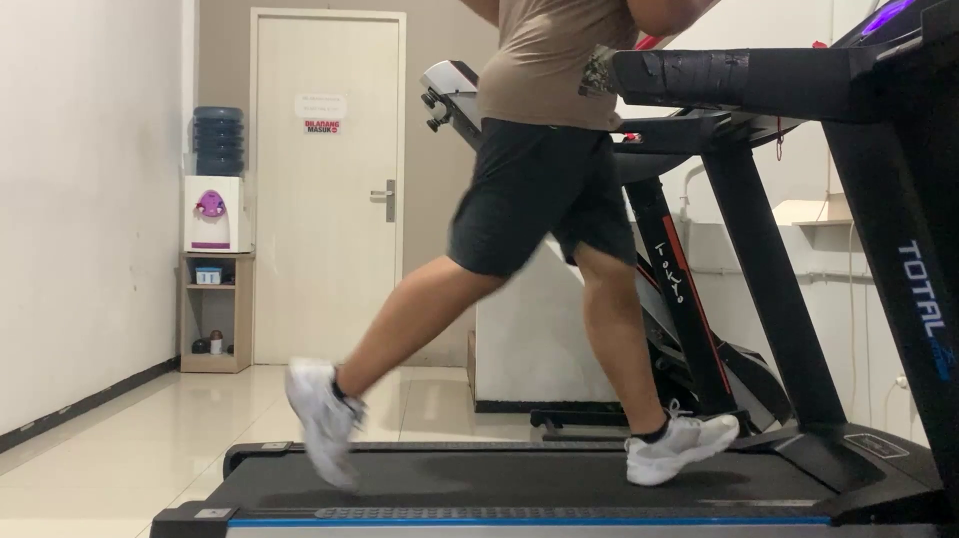
\includegraphics[scale=0.42]{gambar/jarak_dekat.png}
  \caption{Pengujian pada jarak 120 cm}
  \label{fig:PengujianJarakDekat}
\end{figure}

\begin{figure}[H]
  \centering
  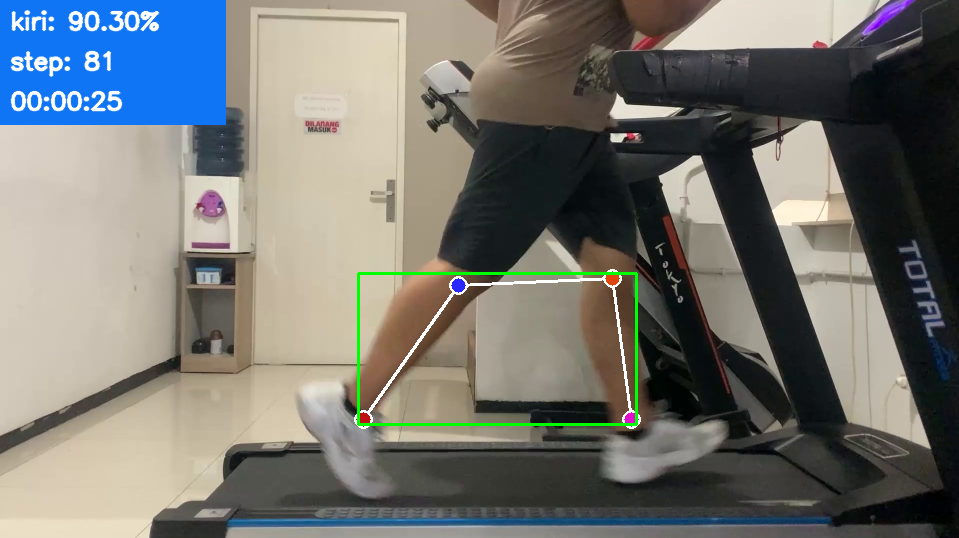
\includegraphics[scale=0.42]{gambar/jarak_dekat2.png}
  \caption{Hasil deteksi pengujian pada jarak 120 cm}
  \label{fig:PengujianJarakDekat2}
\end{figure}

Pengujian dilakukan setelah didapatkan data hasil deteksi yang telah didapat dan juga data sebenarnya berdasarkan hasil perhitungan yang dilakukan terhadap data video. Dengan data video sebagai banyaknya percobaan dilakukan analisa terkait perbandingan hasil yang didapat antara data hasil deteksi dan data perhitungan sebenarnya. Data langkah merupakan data sebagai data sebenarnya atau \emph{actual score} dengan melakukan perhitungan pada data video dan data deteksi langkah sebagai data hasil deteksi langkah yang didapatkan berdasarkan proses deteksi pada sistem. Perbandingan hasil deteksi dengan data sebenarnya dicantumkan pada data eror dan dilakukan persentase berdasarkan data sebenarnya. Hasil persentase eror mendapatkan hasil persentase akurasi yang juga didapatkan berdasarkan persentase eror. Hasil analisa yang didapat dengan melakukan analisa pengujian hasil deteksi didapatkan hasil akurasi rata-rata sebesar 72,37\% dengan hasil eror rata-rata sebesar 27,63\%. Tabel \ref{tb:PengujianJarakDekatAnalisaDeteksi} menunjukkan hasil pengujian dari setiap percobaan yang dilakukan analisa pengujian terhadap hasil deteksi.

\begin{longtable}{|c|c|c|c|c|c|}
  \caption{Hasil Deteksi Pengujian Pada Jarak Dekat}
  \label{tb:PengujianJarakDekatAnalisaDeteksi}                                   \\
  \hline
  \rowcolor[HTML]{C0C0C0}
  \textbf{Percobaan} & \textbf{Langkah} & \textbf{Deteksi Langkah} & \textbf{Eror} & \textbf{Eror\%} & \textbf{Akurasi\%} \\
  \hline
  1   & 255   & 290  & 35  & 13,73\%    & 86,27\%   \\
  \hline
  2   & 254   & 290  & 36  & 14,17\%    & 85,83\%   \\
  \hline
  3   & 265   & 264  & 1   & 0,38\%     & 99,62\%   \\
  \hline
  4   & 327   & 338  & 11  & 3,36\%     & 96,64\%   \\
  \hline
  5   & 311   & 168  & 143 & 45,98\%    & 54,02\%   \\
  \hline
  6   & 322   & 174  & 148 & 45,96\%    & 54,04\%   \\
  \hline
  7   & 271   & 231  & 40  & 14,76\%    & 85,24\%   \\
  \hline
  8   & 254   & 100  & 154 & 60,63\%    & 39,37\%   \\
  \hline
  9   & 292   & 147  & 145 & 49,66\%    & 50,34\%   \\
  \hline

  \multicolumn{4}{|c|}{\textbf{Rata-rata}} & 27,63\% & 72,37\% \\
  \hline
\end{longtable}

Pada pengujian prediksi kalori dilakukan berdasarkan hasil deteksi yang didapat. Hasil deteksi berupa banyaknya langkah, jarak dan waktu tempuh dari data video yang digunakan. Data hasil deteksi akan diilakukan untuk proses prediksi kalori dengan menggunakan model regresi linear yang sudah didapatkan dan menghasilkan data pada prediksi kalori. Analisa pengujian hasil prediksi kalori dilakukan dengan melakukan perbandingan data prediksi kalori dari sistem yang digunakan dengan data kalori treadmill sebagai data sebenarnya atau data \emph{actual score}. Perbandingan hasil prediksi kalori dengan kalori treadmill didapatkan data eror yang kemudian dilakukan perhitungan persentase berdasarkan data sebenarnya pada data kalori treadmill. Proses analisa pengujian dilakukan terhadap seluruh data video pada data percobaan. Hasil analisa yang didapat dengan melakukan analisa pengujian prediksi kalori didapatkan hasil akurasi rata-rata sebesar 49,53\% dengan hasil eror rata-rata sebesar 50,47\%. Tabel \ref{tb:PengujianJarakDekatAnalisaPrediksiRegresi} menunjukkan hasil analisa pengujian dari setiap percobaan yang dilakukan analisa prediksi kalori dengan regresi linear.

\begin{longtable}{|c|c|c|c|c|c|c|c|}
  \caption{Hasil Prediksi Pengujian Pada Jarak Dekat dengan Regresi Linear}
  \label{tb:PengujianJarakDekatAnalisaPrediksiRegresi}                                   \\
  \hline
  \rowcolor[HTML]{C0C0C0}
  & & & & \textbf{Kalori} & \textbf{Prediksi} & & \\
  \rowcolor[HTML]{C0C0C0}
  \multirow{-2}{*}{\textbf{Percobaan}} & \multirow{-2}{*}{\textbf{Langkah}} & \multirow{-2}{*}{\textbf{Jarak}} & \multirow{-2}{*}{\textbf{Waktu}} & \textbf{Treadmill} & \textbf{Kalori} & \multirow{-2}{*}{\textbf{Eror\%}} & \multirow{-2}{*}{\textbf{Akurasi\%}} \\
  
  \hline
  1   & 290   & 163,100    & 2:48    & 10    & 11,364   & 13,64\%      & 86,36\%   \\
  \hline  
  2   & 290   & 163,100    & 1:48    & 10    & 11,364   & 13,64\%      & 86,36\%  \\
  \hline
  3   & 264   & 179,273    & 2:50    & 10    & 12,502   & 25,02\%      & 74,98\%   \\
  \hline
  4   & 338   & 528,603    & 2:03    & 20    & 37,109   & 85,54\%      & 14,46\%  \\
  \hline
  5   & 168   & 106,133    & 2:01    & 20    & 7,368    & 63,16\%      & 36,84\%    \\
  \hline
  6   & 174   & 110,560    & 2:01    & 20    & 7,680    & 61,60\%      & 38,40\%   \\
  \hline
  7   & 231   & 176,116    & 1:39    & 20    & 12,301   & 38,49\%      & 61,51\%   \\
  \hline
  8   & 100   & 46,154     & 1:37    & 20    & 3,315    & 84,23\%      & 15,77\%   \\
  \hline
  9   & 147   & 89,715     & 1:45    & 20    & 6,217    & 68,91\%      & 31,09\%   \\
  \hline

  \multicolumn{6}{|c|}{\textbf{Rata-rata}} & 50,47\% & 49,53\%  \\
  \hline
\end{longtable}

Pada pengujian prediksi kalori dilakukan berdasarkan hasil deteksi yang didapat. Hasil deteksi berupa kecepatan, MET dan waktu tempuh dari data video yang digunakan. Data hasil deteksi akan diilakukan untuk proses prediksi kalori dengan menggunakan perhitungan rumus berdasarkan MET yang sudah didapatkan dan menghasilkan data pada prediksi kalori. Analisa pengujian hasil prediksi kalori dilakukan dengan melakukan perbandingan data prediksi kalori dari sistem yang digunakan dengan data kalori treadmill sebagai data sebenarnya atau data \emph{actual score}. Perbandingan hasil prediksi kalori dengan kalori treadmill didapatkan data eror yang kemudian dilakukan perhitungan persentase berdasarkan data sebenarnya pada data kalori treadmill. Proses analisa pengujian dilakukan terhadap seluruh data video pada data percobaan. Hasil analisa yang didapat dengan melakukan analisa pengujian prediksi kalori didapatkan hasil akurasi rata-rata sebesar 51,87\% dengan hasil eror rata-rata sebesar 48,13\%. Tabel \ref{tb:PengujianJarakDekatAnalisaPrediksiPerhitungan} menunjukkan hasil analisa pengujian dari prediksi kalori dengan perhitungan rumus.

\begin{longtable}{|c|c|c|c|c|c|c|c|}
  \caption{Hasil Prediksi Pengujian Pada Jarak Dekat dengan Perhitungan Rumus}
  \label{tb:PengujianJarakDekatAnalisaPrediksiPerhitungan}                                   \\
  \hline
  \rowcolor[HTML]{C0C0C0}
  & & & & \textbf{Kalori} & \textbf{Prediksi} & & \\
  \rowcolor[HTML]{C0C0C0}
  \multirow{-2}{*}{\textbf{Percobaan}} & \multirow{-2}{*}{\textbf{Kecepatan}} & \multirow{-2}{*}{\textbf{MET}} & \multirow{-2}{*}{\textbf{Waktu}} & \textbf{Treadmill} & \textbf{Kalori} & \multirow{-2}{*}{\textbf{Eror\%}} & \multirow{-2}{*}{\textbf{Akurasi\%}} \\
  \hline
  1   & 3,065   & 4,400    & 2:48    & 10   & 14,014   & 40,14\%     & 67,86\%   \\
  \hline
  2   & 3,065   & 4,400    & 2:48    & 10   & 14,014   & 40,14\%     & 59,86\%   \\
  \hline
  3   & 3,798   & 1,275    & 2:50    & 10   & 4,109    & 58,91\%     & 41,09\%   \\
  \hline
  4   & 14,777  & 13,172   & 2:03    & 20   & 30,715   & 53,58\%      & 46,42\%   \\
  \hline
  5   & 3,115   & 4,170    & 2:01    & 20   & 9,566    & 52,17\%     & 47,83\%   \\
  \hline
  6   & 3,208   & 3,744    & 2:01    & 20   & 8,589    & 57,05\%      & 42,95\%   \\
  \hline
  7   & 6,600   & 6,337    & 1:39    & 20    & 11,893  & 40,53\%      & 59,47\%   \\
  \hline
  8   & 1,195   & 15,325   & 1:37    & 20    & 28,182  & 40,91\%      & 59,09\%   \\
  \hline
  9   & 2,928   & 5,051    & 1:45    & 20    & 10,053  & 49,73\%      & 50,27\%   \\
  \hline

  \multicolumn{6}{|c|}{\textbf{Rata-rata}} & 48,13\% & 51,87\%  \\
  \hline
\end{longtable}


\subsection{Pengujian Pada Jarak Jauh}
\label{subsec:PengujianJarakJauh}

Pengujian dilakukan dengan melakukan pengujian performa sistem pada jarak kamera dekat. Jarak kamera yang digunakan pada pengujian ini dengan jarak 320 cm terhadap objek yang dideteksi. Contoh cuplikan gambar yang memperlihatkan kondisi jarak kamera dekat dengan jaarak 320 cm dapat dilihat pada Gambar \ref{fig:PengujianJarakJauh}. Data percobaan yang digunakan dalam pengujian ini dilakukan proses deteksi dengan sistem yang dibuat untuk dapat melakukan proses estimasi dan deteksi langkah maupun waktu. Proses deteksi yang dilakukan pada data percobaan dapat dilihaat pada Gambar \ref{fig:PengujianJarakJauh2}. Pengujian dilanjutkan dengan melakukan proses prediksi dari hasil deteksi.

\begin{figure}[H]
  \centering
  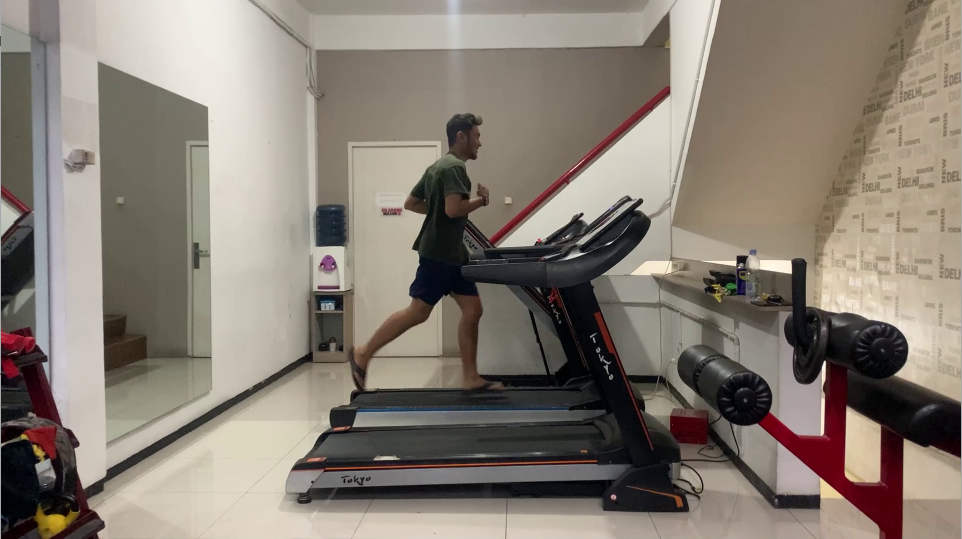
\includegraphics[scale=0.5]{gambar/jarak_jauh.png}
  \caption{Pengujian pada jarak 320 cm}
  \label{fig:PengujianJarakJauh}
\end{figure}

\begin{figure}[H]
  \centering
  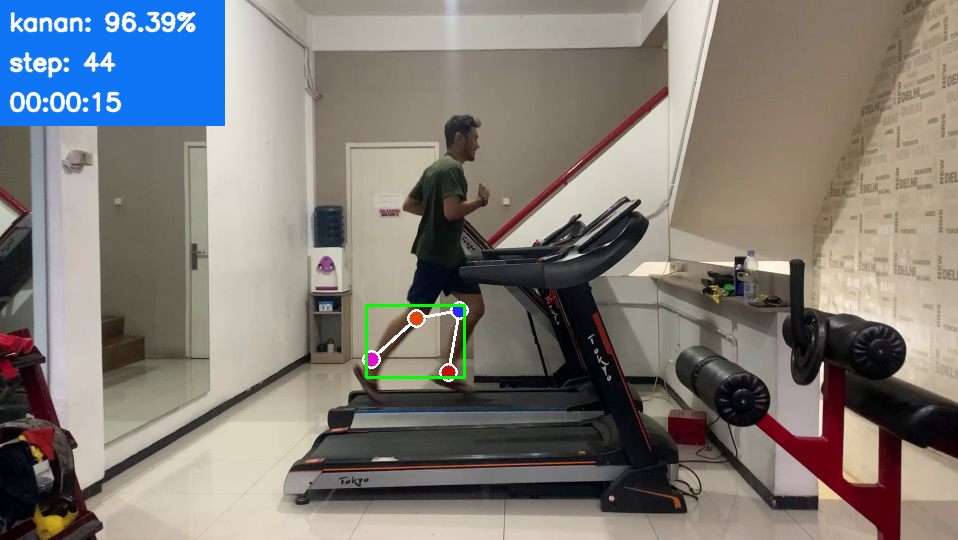
\includegraphics[scale=0.5]{gambar/jarak_jauh2.png}
  \caption{Hasil deteksi pengujian pada jarak 320 cm}
  \label{fig:PengujianJarakJauh2}
\end{figure}

Pengujian dilakukan setelah didapatkan data hasil deteksi yang telah didapat dan juga data sebenarnya berdasarkan hasil perhitungan yang dilakukan terhadap data video. Dengan data video sebagai banyaknya percobaan dilakukan analisa terkait perbandingan hasil yang didapat antara data hasil deteksi dan data perhitungan sebenarnya. Data langkah merupakan data sebagai data sebenarnya atau \emph{actual score} dengan melakukan perhitungan pada data video dan data deteksi langkah sebagai data hasil deteksi langkah yang didapatkan berdasarkan proses deteksi pada sistem. Perbandingan hasil deteksi dengan data sebenarnya dicantumkan pada data eror dan dilakukan persentase berdasarkan data sebenarnya. Hasil persentase eror mendapatkan hasil persentase akurasi yang juga didapatkan berdasarkan persentase eror. Hasil analisa yang didapat dengan melakukan analisa pengujian hasil deteksi didapatkan hasil akurasi rata-rata sebesar 82,59\% dengan hasil eror rata-rata sebesar 17,41\%. Tabel \ref{tb:PengujianJarakJauhAnalisaDeteksi} menunjukkan hasil pengujian dari setiap percobaan yang dilakukan analisa pengujian terhadap hasil deteksi.

\begin{longtable}{|c|c|c|c|c|c|}
  \caption{Hasil Deteksi Pengujian Pada Jarak Jauh}
  \label{tb:PengujianJarakJauhAnalisaDeteksi}                                   \\
  \hline
  \rowcolor[HTML]{C0C0C0}
  \textbf{Percobaan} & \textbf{Langkah} & \textbf{Deteksi Langkah} & \textbf{Eror} & \textbf{Eror\%} & \textbf{Akurasi\%} \\
  \hline
  1   & 255   & 336 & 81   & 31,76\%    & 68,24\%   \\
  \hline
  2   & 254   & 268 & 14   & 5,51\%     & 94,49\%   \\
  \hline
  3   & 265   & 269 & 4    & 1,51\%     & 98,49\%     \\
  \hline
  4   & 327   & 284 & 43   & 13,15\%    & 86,85\%   \\
  \hline
  5   & 311   & 302 & 9    & 2,89\%     & 97,11\%   \\
  \hline
  6   & 322   & 204 & 118  & 36,65\%    & 63,35\%   \\
  \hline
  7   & 271   & 224 & 47   & 17,34\%    & 82,66\%   \\
  \hline
  8   & 254   & 236 & 18   & 7,09\%     & 92,91\%   \\
  \hline
  9   & 292   & 173 & 119  & 40,75\%   & 59,25\%   \\
  \hline

  \multicolumn{4}{|c|}{\textbf{Rata-rata}} & 17,41\% & 82,59\% \\
  \hline
\end{longtable}

Pada pengujian prediksi kalori dilakukan berdasarkan hasil deteksi yang didapat. Hasil deteksi berupa banyaknya langkah, jarak dan waktu tempuh dari data video yang digunakan. Data hasil deteksi akan diilakukan untuk proses prediksi kalori dengan menggunakan model regresi linear yang sudah didapatkan dan menghasilkan data pada prediksi kalori. Analisa pengujian hasil prediksi kalori dilakukan dengan melakukan perbandingan data prediksi kalori dari sistem yang digunakan dengan data kalori treadmill sebagai data sebenarnya atau data \emph{actual score}. Perbandingan hasil prediksi kalori dengan kalori treadmill didapatkan data eror yang kemudian dilakukan perhitungan persentase berdasarkan data sebenarnya pada data kalori treadmill. Proses analisa pengujian dilakukan terhadap seluruh data video pada data percobaan. Hasil analisa yang didapat dengan melakukan analisa pengujian prediksi kalori didapatkan hasil akurasi rata-rata sebesar 63,80\% dengan hasil eror rata-rata sebesar 36,20\%. Tabel \ref{tb:PengujianJarakJauhAnalisaPrediksiRegresi} menunjukkan hasil analisa pengujian dari setiap percobaan yang dilakukan analisa prediksi kalori dengan regresi linear.

\begin{longtable}{|c|c|c|c|c|c|c|c|}
  \caption{Hasil Prediksi Pengujian Pada Jarak Jauh dengan Regresi Linear}
  \label{tb:PengujianJarakJauhAnalisaPrediksiRegresi}                                   \\
  \hline
  \rowcolor[HTML]{C0C0C0}
  & & & & \textbf{Kalori} & \textbf{Prediksi} & & \\
  \rowcolor[HTML]{C0C0C0}
  \multirow{-2}{*}{\textbf{Percobaan}} & \multirow{-2}{*}{\textbf{Langkah}} & \multirow{-2}{*}{\textbf{Jarak}} & \multirow{-2}{*}{\textbf{Waktu}} & \textbf{Treadmill} & \textbf{Kalori} & \multirow{-2}{*}{\textbf{Eror\%}} & \multirow{-2}{*}{\textbf{Akurasi\%}} \\
  
  \hline
  1   & 336   & 97,956     & 2:48    & 10    & 6,778    & 32,22\%      & 67,78\%   \\
  \hline  
  2   & 268   & 175,943    & 2:48    & 10    & 12,268   & 22,68\%      & 77,32\%  \\
  \hline
  3   & 269   & 178,949    & 2:50    & 10    & 12,479   & 24,79\%      & 75,21\%   \\
  \hline
  4   & 284   & 166,973    & 2:03    & 20    & 11,650   & 41,75\%      & 58,25\%  \\
  \hline
  5   & 302   & 252,115    & 2:01    & 20    & 17,645   & 11,77\%      & 88,23\%    \\
  \hline
  6   & 204   & 123,654    & 2:01    & 20    & 8,601    & 56,99\%      & 43,01\%   \\
  \hline
  7   & 224   & 160,596    & 1:39    & 20    & 11,209   & 43,95\%      & 56,05\%   \\
  \hline
  8   & 236   & 203,020    & 1:37    & 20    & 14,196   & 29,02\%      & 70,98\%   \\
  \hline
  9   & 173   & 107,558    & 1:45    & 20    & 7,473    & 62,63\%      & 37,37\%   \\
  \hline

  \multicolumn{6}{|c|}{\textbf{Rata-rata}} & 36,20\% & 63,80\% \\
  \hline
\end{longtable}

Pada pengujian prediksi kalori dilakukan berdasarkan hasil deteksi yang didapat. Hasil deteksi berupa kecepatan, MET dan waktu tempuh dari data video yang digunakan. Data hasil deteksi akan diilakukan untuk proses prediksi kalori dengan menggunakan perhitungan rumus berdasarkan MET yang sudah didapatkan dan menghasilkan data pada prediksi kalori. Analisa pengujian hasil prediksi kalori dilakukan dengan melakukan perbandingan data prediksi kalori dari sistem yang digunakan dengan data kalori treadmill sebagai data sebenarnya atau data \emph{actual score}. Perbandingan hasil prediksi kalori dengan kalori treadmill didapatkan data eror yang kemudian dilakukan perhitungan persentase berdasarkan data sebenarnya pada data kalori treadmill. Proses analisa pengujian dilakukan terhadap seluruh data video pada data percobaan. Hasil analisa yang didapat dengan melakukan analisa pengujian prediksi kalori didapatkan hasil akurasi rata-rata sebesar 47,78\% dengan hasil eror rata-rata sebesar 52,22\%. Tabel \ref{tb:PengujianJarakJauhAnalisaPrediksiPerhitungan} menunjukkan hasil analisa pengujian dari prediksi kalori dengan perhitungan rumus.

\begin{longtable}{|c|c|c|c|c|c|c|c|}
  \caption{Hasil Prediksi Pengujian Pada Jarak Jauh dengan Perhitungan Rumus}
  \label{tb:PengujianJarakJauhAnalisaPrediksiPerhitungan}                                   \\
  \hline
  \rowcolor[HTML]{C0C0C0}
  & & & & \textbf{Kalori} & \textbf{Prediksi} & & \\
  \rowcolor[HTML]{C0C0C0}
  \multirow{-2}{*}{\textbf{Percobaan}} & \multirow{-2}{*}{\textbf{Kecepatan}} & \multirow{-2}{*}{\textbf{MET}} & \multirow{-2}{*}{\textbf{Waktu}} & \textbf{Treadmill} & \textbf{Kalori} & \multirow{-2}{*}{\textbf{Eror\%}} & \multirow{-2}{*}{\textbf{Akurasi\%}} \\
  \hline
  1   & 1,387   & 5,740    & 2:48    & 10   & 18,281   & 82,81\%     & 17,19\%   \\
  \hline
  2   & 3,657   & 1,835    & 2:48    & 10   & 5,844    & 41,56\%     & 58,44\%   \\
  \hline
  3   & 3,717   & 1,593    & 2:50    & 10   & 5,135    & 48,65\%     & 51,35\%   \\
  \hline
  4   & 4,906   & 2,454    & 2:03    & 20   & 5,722    & 71,39\%     & 28,61\%   \\
  \hline
  5   & 7,666   & 7,946    & 2:01    & 20   & 18,227   & 8,86\%      & 91,14\%   \\
  \hline
  6   & 3,371   & 3,027    & 2:01    & 20   & 6,944    & 65,28\%     & 34,72\%   \\
  \hline
  7   & 5,978   & 5,128    & 1:39    & 20   & 9,625    & 51,88\%     & 48,12\%   \\
  \hline
  8   & 7,786   & 8,097    & 1:37    & 20   & 14,890   & 25,55\%     & 74,45\%   \\
  \hline
  9   & 3,469   & 2,611    & 1:45    & 20   & 5,197    & 74,02\%     & 25,98\%   \\
  \hline

  \multicolumn{6}{|c|}{\textbf{Rata-rata}} & 52,22\% & 47,78\%  \\
  \hline
\end{longtable}

Berdasarkan pengujian yang telah dilakukan terhadap hasil performa deteksi langkah, prediksi kalori dengan regresi dan prediksi kalori dengan perhitungan rumus didapatkan hasil performa dalam nilai akurasi rata-rata dan eror rata-rata dari setiap pengujian. Pada pengujian deteksi langkah didapatkan akurasi rata-rata lebih baik pada jarak kamera 320 cm dengan nilai akurasi rata-rata sebesar 82,59\% sedangkan pada jarak kamera 120 cm didapat nilai akurasi rata-rata sebesar 72,37\%. Pada pengujian prediksi kalori dengan regresi didapatkan akurasi rata-rata lebih baik pada jarak kamera 320 cm dengan nilai akurasi rata-rata sebesar 63,80\% sedangkan pada jarak kamera 120 cm didapat nilai akurasi rata-rata sebesar 49,53\%. Pada pengujian prediksi kalori dengan perhitungan rumus didapatkan akurasi rata-rata lebih baik pada jarak kamera 120 cm dengan nilai akurasi rata-rata sebesar 51,87\% sedangkan pada jarak kamera 320 cm didapat nilai akurasi rata-rata sebesar 47,78\%. Gambar \ref{fig:DiagramJarak} menunjukkan diagram perbandingan performa pengujian dengan nilai akurasi rata-rata berdasarkan jarak kamera.

\begin{figure}[H]
  \centering
  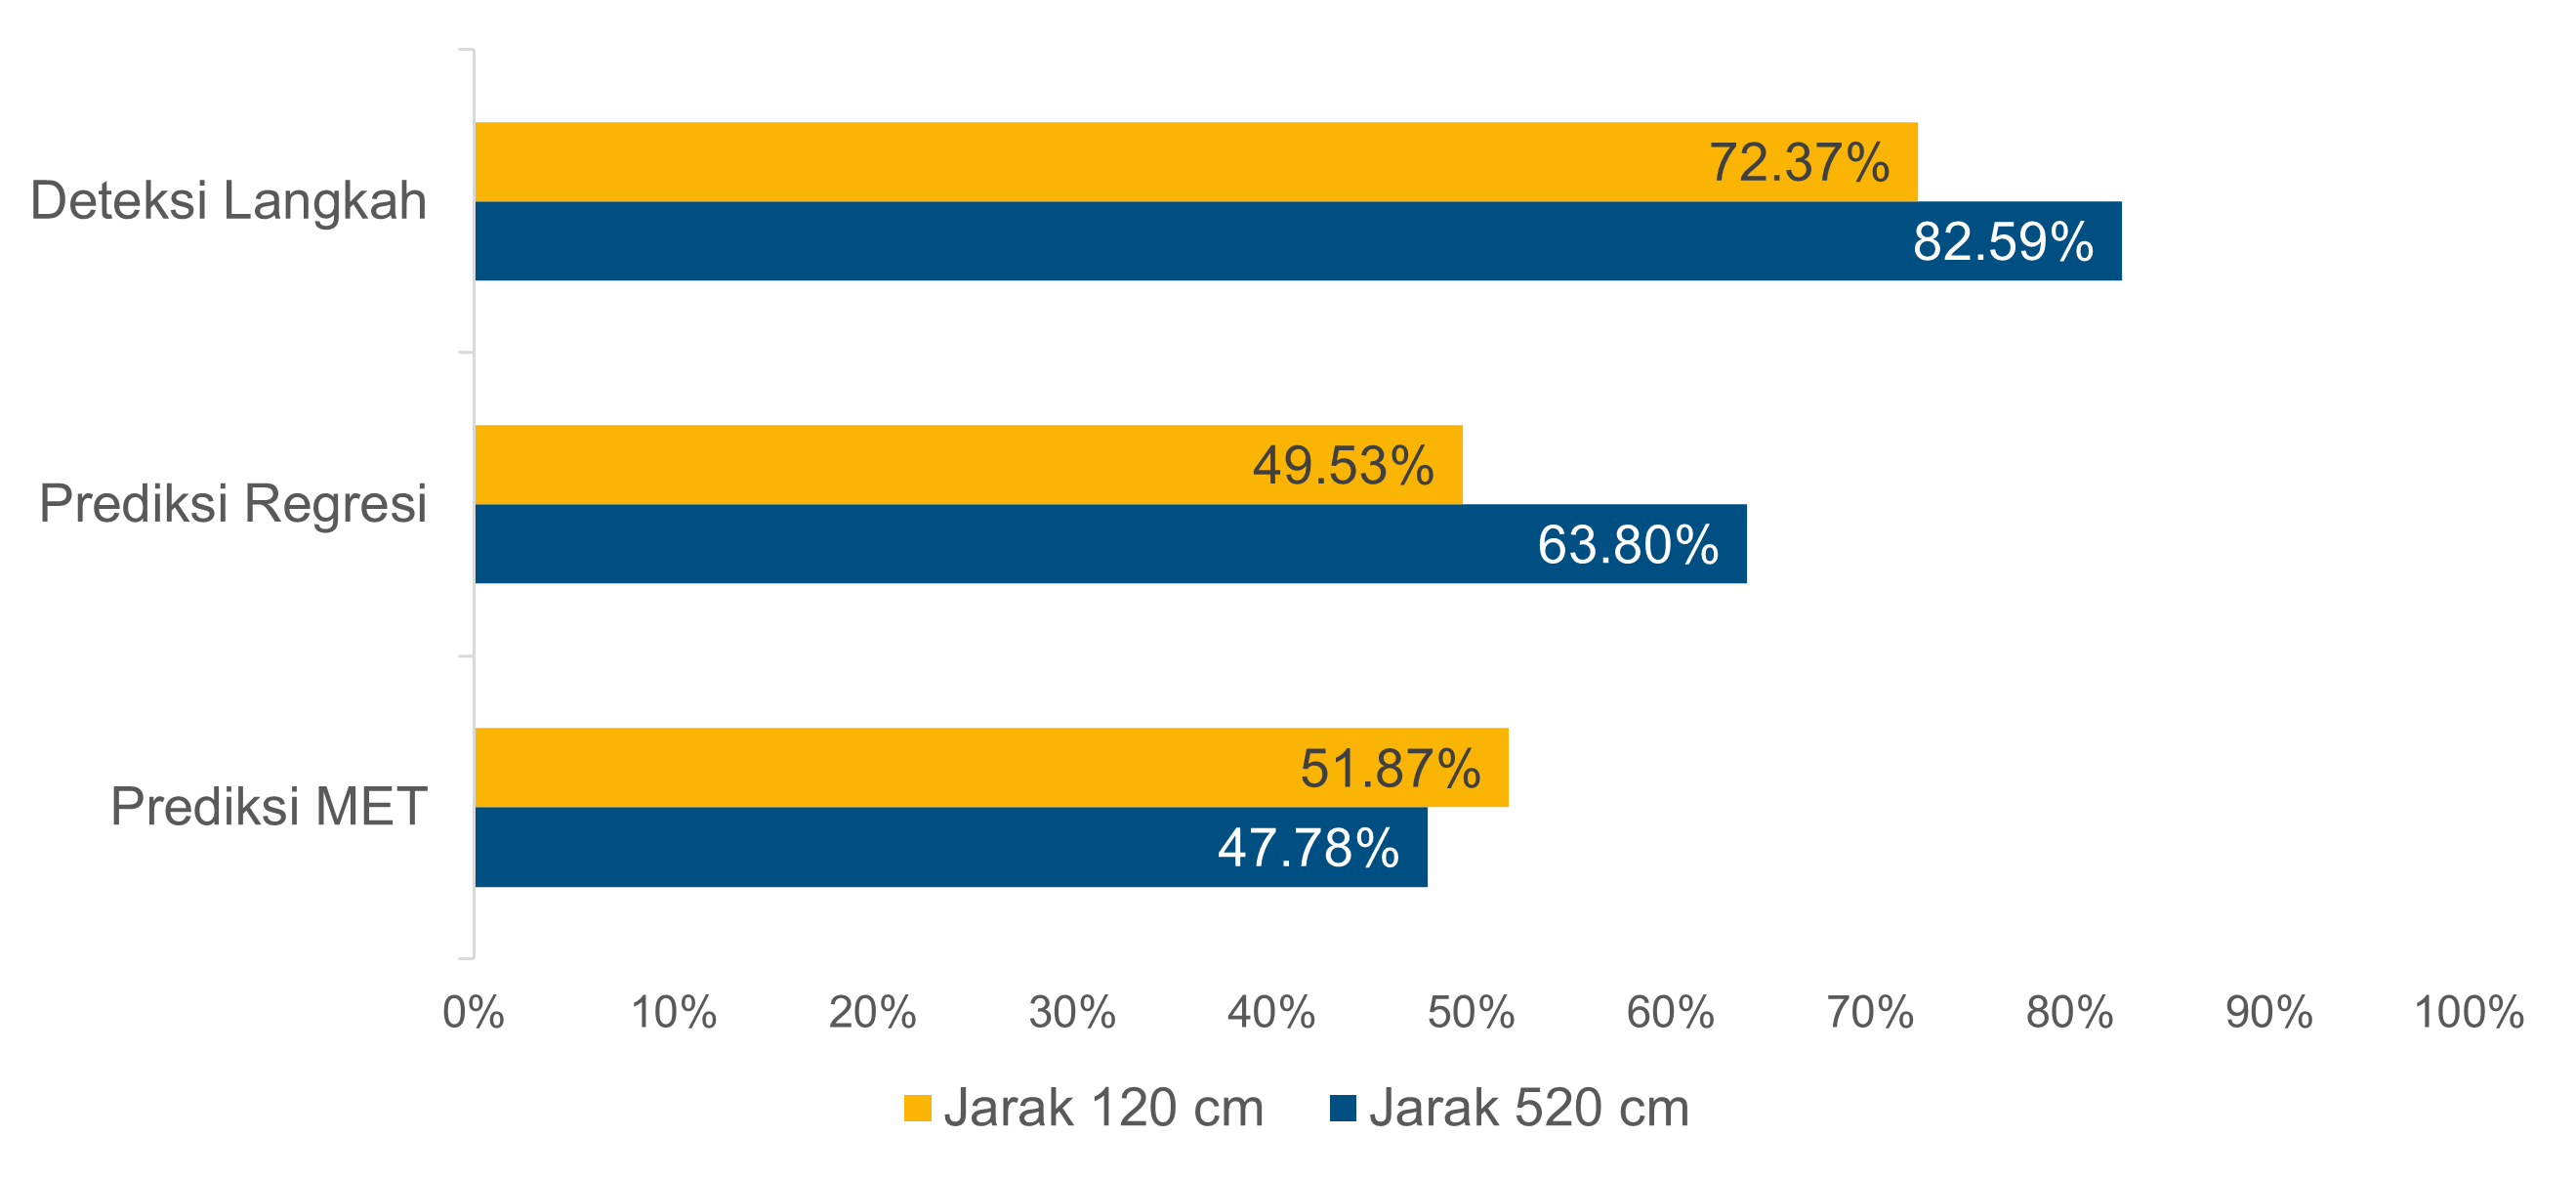
\includegraphics[scale=0.7]{gambar/diagram_jarak.png}
  \caption{Diagram perbandingan performa berdasarkan jarak kamera}
  \label{fig:DiagramJarak}
\end{figure}

\section{Pengujian Performa Berdasarkan Posisi Kamera}
\label{sec:PengujianPosisi}

Pada pengujian ini dilakukan deteksi dan prediksi kalori dengan menggunakan skenario berdasarkan posisi kamera terhdap objek deteksi yang berbeda-beda. Skenario pertama yang dilakukan adalah pengujian pada posisi kamera serong, posisi kamera berada di arah samping yang sedikit di arah depan dari objek yang terlihat dengan sudut 45 derajat dari samping objek sehingga terlihat sebagian wajah dari objek yang akan dilakukan deteksi. Skenario kedua yang dilakukan adalah pengujian pada posisi kamera belakang, posisi kamera berada di arah belakang dari objek sehingga terlihat bagian belakang objek yang akan dilakukan deteksi. Video pengujian yang digunakan dengan banyak percobaan sebanyak 9 kali dengan menggunakan variasi kecepatan dan hasil kalori yang didapatkan. Variasi kecepatan yang digunakan adalah 3 km/jam, 9 km/jam dan 12 km/jam. Kemudian variasi hasil kalori yang didapatkan adalah 10 dan 20 kcal. 


\subsection{Pengujian Pada Posisi Serong}
\label{subsec:PengujianPosisiSerong}

Pengujian dilakukan dengan melakukan pengujian performa sistem pada posisi kamera serong. Posisi kamera yang digunakan pada pengujian ini dengan posisi serong dengan sudut 45 derajat dari samping objek yang dilakukan deteksi. Contoh cuplikan gambar yang memperlihatkan kondisi posisi kamera serong dapat dilihat pada Gambar \ref{fig:PengujianPosisiSerong}. Data percobaan yang digunakan dalam pengujian ini dilakukan proses deteksi dengan sistem yang dibuat untuk dapat melakukan proses estimasi dan deteksi langkah maupun waktu. Proses deteksi yang dilakukan pada data percobaan dapat dilihaat pada Gambar \ref{fig:PengujianPosisiSerong2}. Pengujian dilanjutkan dengan melakukan proses prediksi dari hasil deteksi.

\begin{figure}[H]
  \centering
  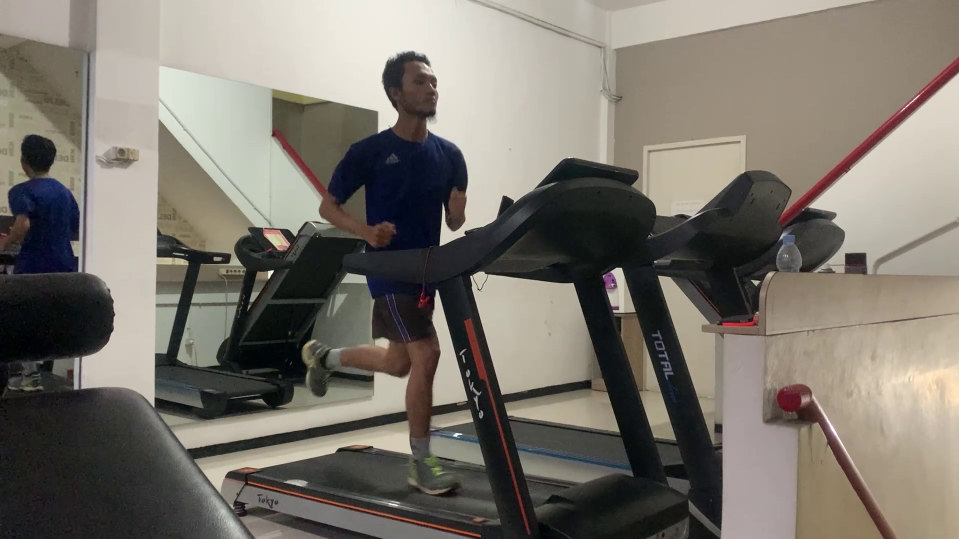
\includegraphics[scale=0.5]{gambar/posisi_serong.png}
  \caption{Pengujian pada posisi serong}
  \label{fig:PengujianPosisiSerong}
\end{figure}

\begin{figure}[H]
  \centering
  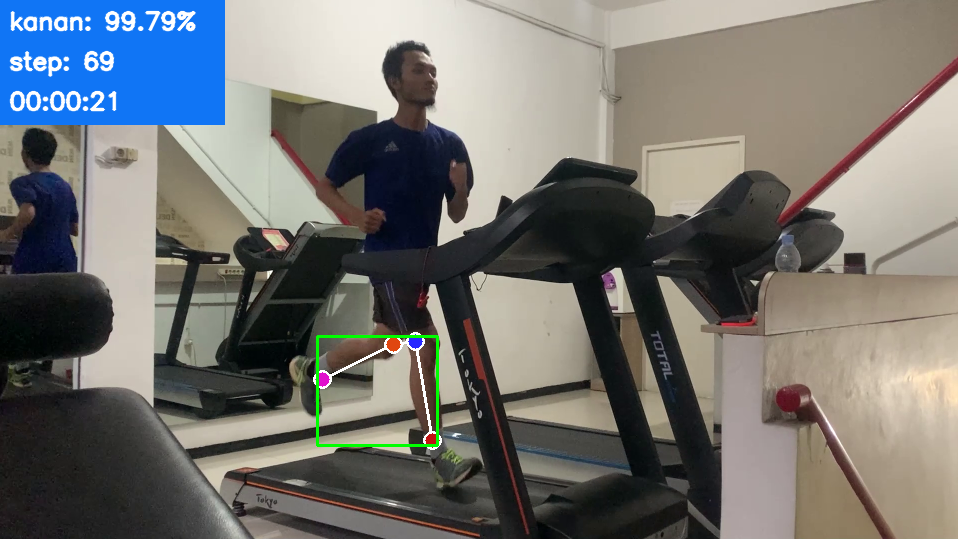
\includegraphics[scale=0.5]{gambar/posisi_serong2.png}
  \caption{Hasil deteksi pengujian pada posisi serong}
  \label{fig:PengujianPosisiSerong2}
\end{figure}

Pengujian dilakukan setelah didapatkan data hasil deteksi yang telah didapat dan juga data sebenarnya berdasarkan hasil perhitungan yang dilakukan terhadap data video. Dengan data video sebagai banyaknya percobaan dilakukan analisa terkait perbandingan hasil yang didapat antara data hasil deteksi dan data perhitungan sebenarnya. Data langkah merupakan data sebagai data sebenarnya atau \emph{actual score} dengan melakukan perhitungan pada data video dan data deteksi langkah sebagai data hasil deteksi langkah yang didapatkan berdasarkan proses deteksi pada sistem. Perbandingan hasil deteksi dengan data sebenarnya dicantumkan pada data eror dan dilakukan persentase berdasarkan data sebenarnya. Hasil persentase eror mendapatkan hasil persentase akurasi yang juga didapatkan berdasarkan persentase eror. Hasil analisa yang didapat dengan melakukan analisa pengujian hasil deteksi didapatkan hasil akurasi rata-rata sebesar 86,80\% dengan hasil eror rata-rata sebesar 13,20\%. Tabel \ref{tb:PengujianPosisiSerongAnalisaDeteksi} menunjukkan hasil pengujian dari setiap percobaan yang dilakukan analisa pengujian terhadap hasil deteksi.

\begin{longtable}{|c|c|c|c|c|c|}
  \caption{Hasil Deteksi Pengujian Pada Posisi Serong}
  \label{tb:PengujianPosisiSerongAnalisaDeteksi}                                   \\
  \hline
  \rowcolor[HTML]{C0C0C0}
  \textbf{Percobaan} & \textbf{Langkah} & \textbf{Deteksi Langkah} & \textbf{Eror} & \textbf{Eror\%} & \textbf{Akurasi\%} \\
  \hline
  1   & 226   & 221  & 5   & 2,21\%    & 97,79\%   \\
  \hline
  2   & 236   & 207  & 29  & 12,29\%   & 87,71\%   \\
  \hline
  3   & 241   & 213  & 28  & 11,62\%   & 88,38\%   \\
  \hline
  4   & 371   & 357  & 14  & 3,77\%    & 96,23\%   \\
  \hline
  5   & 350   & 334  & 16  & 4,57\%    & 95,43\%   \\
  \hline
  6   & 359   & 291  & 68  & 18,94\%   & 81,06\%   \\
  \hline
  7   & 281   & 267  & 14  & 4,98\%    & 95,02\%   \\
  \hline
  8   & 267   & 192  & 75  & 28,09\%   & 71,91\%   \\
  \hline
  9   & 294   & 199  & 95  & 32,31\%   & 67,69\%   \\
  \hline

  \multicolumn{4}{|c|}{\textbf{Rata-rata}} & 13,20\% & 86,80\% \\
  \hline
\end{longtable}

Pada pengujian prediksi kalori dilakukan berdasarkan hasil deteksi yang didapat. Hasil deteksi berupa banyaknya langkah, jarak dan waktu tempuh dari data video yang digunakan. Data hasil deteksi akan diilakukan untuk proses prediksi kalori dengan menggunakan model regresi linear yang sudah didapatkan dan menghasilkan data pada prediksi kalori. Analisa pengujian hasil prediksi kalori dilakukan dengan melakukan perbandingan data prediksi kalori dari sistem yang digunakan dengan data kalori treadmill sebagai data sebenarnya atau data \emph{actual score}. Perbandingan hasil prediksi kalori dengan kalori treadmill didapatkan data eror yang kemudian dilakukan perhitungan persentase berdasarkan data sebenarnya pada data kalori treadmill. Proses analisa pengujian dilakukan terhadap seluruh data video pada data percobaan. Hasil analisa yang didapat dengan melakukan analisa pengujian prediksi kalori didapatkan hasil akurasi rata-rata sebesar 70,18\% dengan hasil eror rata-rata sebesar 29,82\%. Tabel \ref{tb:PengujianPosisiSerongAnalisaPrediksiRegresi} menunjukkan hasil analisa pengujian dari setiap percobaan yang dilakukan analisa prediksi kalori dengan regresi linear.

\begin{longtable}{|c|c|c|c|c|c|c|c|}
  \caption{Hasil Prediksi Pengujian Pada Posisi Serong dengan Regresi Linear}
  \label{tb:PengujianPosisiSerongAnalisaPrediksiRegresi}                                   \\
  \hline
  \rowcolor[HTML]{C0C0C0}
  & & & & \textbf{Kalori} & \textbf{Prediksi} & & \\
  \rowcolor[HTML]{C0C0C0}
  \multirow{-2}{*}{\textbf{Percobaan}} & \multirow{-2}{*}{\textbf{Langkah}} & \multirow{-2}{*}{\textbf{Jarak}} & \multirow{-2}{*}{\textbf{Waktu}} & \textbf{Treadmill} & \textbf{Kalori} & \multirow{-2}{*}{\textbf{Eror\%}} & \multirow{-2}{*}{\textbf{Akurasi\%}} \\
  
  \hline
  1   & 221   & 136,365    & 2:15    & 10    & 9,492    & 5,08\%      & 94,92\%   \\
  \hline  
  2   & 207   & 132,305    & 2:13    & 10    & 9,207    & 7,93\%      & 92,07\%  \\
  \hline
  3   & 213   & 133,706    & 2:16    & 10    & 9,305    & 6,95\%      & 93,05\%   \\
  \hline
  4   & 357   & 579,448    & 2:10    & 20    & 17,249   & 13,75\%     & 86,25\%  \\
  \hline
  5   & 334   & 324,206    & 2:10    & 20    & 10,165   & 49,17\%     & 50,83\%    \\
  \hline
  6   & 291   & 143,608    & 2:11    & 20    & 8,154    & 59,23\%     & 40,77\%   \\
  \hline
  7   & 267   & 259,668    & 1:45    & 20    & 18,182   & 9,09\%      & 90,91\%   \\
  \hline
  8   & 192   & 117,049    & 1:46    & 20    & 11,859   & 59,29\%     & 40,71\%   \\
  \hline
  9   & 199   & 120,996    & 1:45    & 20    & 11,581   & 57,90\%     & 42,10\%   \\
  \hline

  \multicolumn{6}{|c|}{\textbf{Rata-rata}} & 29,82\% & 70,18\%  \\
  \hline
\end{longtable}

Pada pengujian prediksi kalori dilakukan berdasarkan hasil deteksi yang didapat. Hasil deteksi berupa kecepatan, MET dan waktu tempuh dari data video yang digunakan. Data hasil deteksi akan diilakukan untuk proses prediksi kalori dengan menggunakan perhitungan rumus berdasarkan MET yang sudah didapatkan dan menghasilkan data pada prediksi kalori. Analisa pengujian hasil prediksi kalori dilakukan dengan melakukan perbandingan data prediksi kalori dari sistem yang digunakan dengan data kalori treadmill sebagai data sebenarnya atau data \emph{actual score}. Perbandingan hasil prediksi kalori dengan kalori treadmill didapatkan data eror yang kemudian dilakukan perhitungan persentase berdasarkan data sebenarnya pada data kalori treadmill. Proses analisa pengujian dilakukan terhadap seluruh data video pada data percobaan. Hasil analisa yang didapat dengan melakukan analisa pengujian prediksi kalori didapatkan hasil akurasi rata-rata sebesar 53,20\% dengan hasil eror rata-rata sebesar 46,80\%. Tabel \ref{tb:PengujianPosisiSerongAnalisaPrediksiPerhitungan} menunjukkan hasil analisa pengujian dari prediksi kalori dengan perhitungan rumus.

\begin{longtable}{|c|c|c|c|c|c|c|c|}
  \caption{Hasil Prediksi Pengujian Pada Posisi Serong dengan Perhitungan Rumus}
  \label{tb:PengujianPosisiSerongAnalisaPrediksiPerhitungan}                                   \\
  \hline
  \rowcolor[HTML]{C0C0C0}
  & & & & \textbf{Kalori} & \textbf{Prediksi} & & \\
  \rowcolor[HTML]{C0C0C0}
  \multirow{-2}{*}{\textbf{Percobaan}} & \multirow{-2}{*}{\textbf{Kecepatan}} & \multirow{-2}{*}{\textbf{MET}} & \multirow{-2}{*}{\textbf{Waktu}} & \textbf{Treadmill} & \textbf{Kalori} & \multirow{-2}{*}{\textbf{Eror\%}} & \multirow{-2}{*}{\textbf{Akurasi\%}} \\
  \hline
  1   & 3,357   & 3,088    & 2:15    & 10   & 7,903     & 20,97\%     & 79,03\%   \\
  \hline
  2   & 3,416   & 2,834    & 2:13    & 10   & 7,145     & 28,55\%     & 71,45\%   \\
  \hline
  3   & 3,434   & 2,758    & 2:16    & 10   & 7,110     & 28,90\%     & 71,10\%   \\
  \hline
  4   & 15,216  & 13,542   & 2:10    & 20   & 33,376    & 66,88\%     & 33,12\%   \\
  \hline
  5   & 9,034   & 9,380    & 2:10    & 20   & 23,118    & 15,59\%     & 84,41\%   \\
  \hline
  6   & 3,660   & 1,821    & 2:10    & 20   & 4,521     & 77,39\%     & 22,61\%   \\
  \hline
  7   & 9,095   & 9,432    & 1:45    & 20    & 18,775   & 6,12\%      & 93,88\%   \\
  \hline
  8   & 3,729   & 1,547    & 1:46    & 20    & 3,109    & 84,45\%     & 15,55\%   \\
  \hline
  9   & 3,931   & 0,770    & 1:45    & 20    & 1,532    & 92,34\%     & 7,66\%   \\
  \hline

  \multicolumn{6}{|c|}{\textbf{Rata-rata}} & 46,80\% & 53,20\%  \\
  \hline
\end{longtable}

\subsection{Pengujian Pada Posisi Belakang}
\label{subsec:PengujianPosisiBelakang}

Pengujian dilakukan dengan melakukan pengujian performa sistem pada posisi kamera serong. Posisi kamera yang digunakan pada pengujian ini dengan posisi belakang dengan terlihat bagian belakang objek yang dilakukan deteksi. Contoh cuplikan gambar yang memperlihatkan kondisi posisi kamera belakang dapat dilihat pada Gambar \ref{fig:PengujianPosisiBelakang}. Data percobaan yang digunakan dalam pengujian ini dilakukan proses deteksi dengan sistem yang dibuat untuk dapat melakukan proses estimasi dan deteksi langkah maupun waktu. Proses deteksi yang dilakukan pada data percobaan dapat dilihaat pada Gambar \ref{fig:PengujianPosisiBelakang2}. Pengujian dilanjutkan dengan melakukan proses prediksi dari hasil deteksi.

\begin{figure}[H]
  \centering
  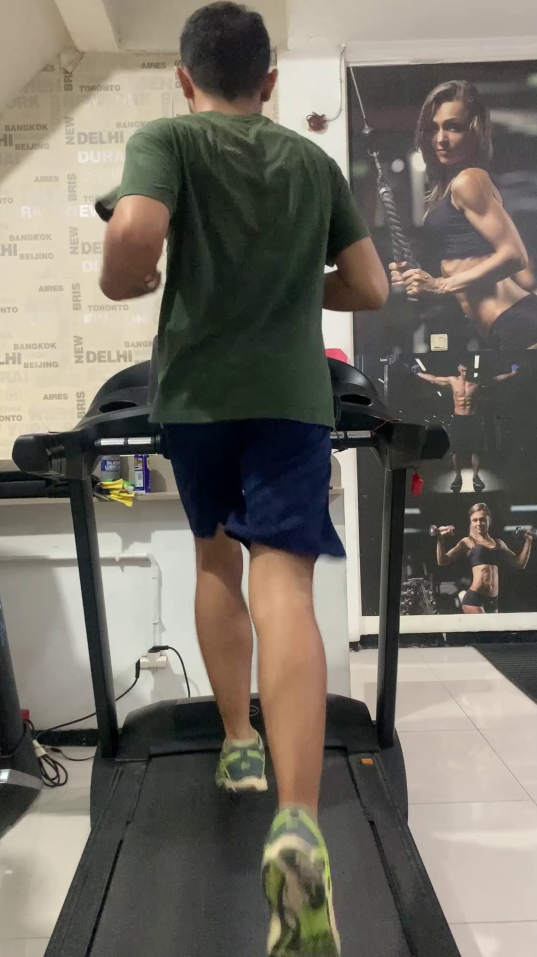
\includegraphics[scale=0.4]{gambar/posisi_belakang.png}
  \caption{Pengujian pada posisi belakang}
  \label{fig:PengujianPosisiBelakang}
\end{figure}

\begin{figure}[H]
  \centering
  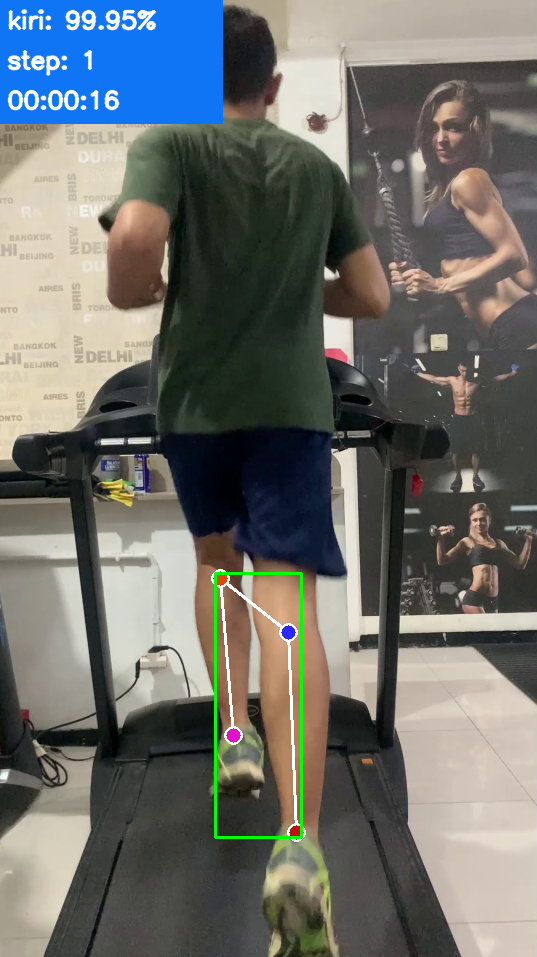
\includegraphics[scale=0.4]{gambar/posisi_belakang2.png}
  \caption{Hasil deteksi pengujian pada posisi belakang}
  \label{fig:PengujianPosisiBelakang2}
\end{figure}

Pengujian dilakukan setelah didapatkan data hasil deteksi yang telah didapat dan juga data sebenarnya berdasarkan hasil perhitungan yang dilakukan terhadap data video. Dengan data video sebagai banyaknya percobaan dilakukan analisa terkait perbandingan hasil yang didapat antara data hasil deteksi dan data perhitungan sebenarnya. Data langkah merupakan data sebagai data sebenarnya atau \emph{actual score} dengan melakukan perhitungan pada data video dan data deteksi langkah sebagai data hasil deteksi langkah yang didapatkan berdasarkan proses deteksi pada sistem. Perbandingan hasil deteksi dengan data sebenarnya dicantumkan pada data eror dan dilakukan persentase berdasarkan data sebenarnya. Hasil persentase eror mendapatkan hasil persentase akurasi yang juga didapatkan berdasarkan persentase eror. Hasil analisa yang didapat dengan melakukan analisa pengujian hasil deteksi didapatkan hasil akurasi rata-rata sebesar 67,23\% dengan hasil eror rata-rata sebesar 32,77\%. Tabel \ref{tb:PengujianPosisiBelakangAnalisaDeteksi} menunjukkan hasil pengujian dari setiap percobaan yang dilakukan analisa pengujian terhadap hasil deteksi.

\begin{longtable}{|c|c|c|c|c|c|}
  \caption{Hasil Deteksi Pengujian Pada Posisi Belakang}
  \label{tb:PengujianPosisiBelakangAnalisaDeteksi}                                   \\
  \hline
  \rowcolor[HTML]{C0C0C0}
  \textbf{Percobaan} & \textbf{Langkah} & \textbf{Deteksi Langkah} & \textbf{Eror} & \textbf{Eror\%} & \textbf{Akurasi\%} \\
  \hline
  1   & 234   & 194  & 40   & 17,09\%    & 82,91\%   \\
  \hline
  2   & 235   & 150  & 85   & 36,17\%    & 63,83\%   \\
  \hline
  3   & 249   & 236  & 13   & 5,22\%     & 94,78\%   \\
  \hline
  4   & 361   & 92   & 269  & 74,52\%    & 25,48\%   \\
  \hline
  5   & 345   & 234  & 111  & 32,17\%    & 67,83\%   \\
  \hline
  6   & 343   & 272  & 71   & 20,70\%    & 79,30\%   \\
  \hline
  7   & 276   & 138  & 138  & 50\%       & 50\%   \\
  \hline
  8   & 267   & 192  & 75   & 28,09\%    & 71,91\%   \\
  \hline
  9   & 284   & 196  & 88   & 30,99\%    & 69,07\%   \\
  \hline

  \multicolumn{4}{|c|}{\textbf{Rata-rata}} & 32,77\% & 67,23\% \\
  \hline
\end{longtable}

Pada pengujian prediksi kalori dilakukan berdasarkan hasil deteksi yang didapat. Hasil deteksi berupa banyaknya langkah, jarak dan waktu tempuh dari data video yang digunakan. Data hasil deteksi akan diilakukan untuk proses prediksi kalori dengan menggunakan model regresi linear yang sudah didapatkan dan menghasilkan data pada prediksi kalori. Analisa pengujian hasil prediksi kalori dilakukan dengan melakukan perbandingan data prediksi kalori dari sistem yang digunakan dengan data kalori treadmill sebagai data sebenarnya atau data \emph{actual score}. Perbandingan hasil prediksi kalori dengan kalori treadmill didapatkan data eror yang kemudian dilakukan perhitungan persentase berdasarkan data sebenarnya pada data kalori treadmill. Proses analisa pengujian dilakukan terhadap seluruh data video pada data percobaan. Hasil analisa yang didapat dengan melakukan analisa pengujian prediksi kalori didapatkan hasil akurasi rata-rata sebesar 49,86\% dengan hasil eror rata-rata sebesar 50,14\%. Tabel \ref{tb:PengujianPosisiBelakangAnalisaPrediksiRegresi} menunjukkan hasil analisa pengujian dari setiap percobaan yang dilakukan analisa prediksi kalori dengan regresi linear.

\begin{longtable}{|c|c|c|c|c|c|c|c|}
  \caption{Hasil Prediksi Pengujian Pada Posisi Belakang dengan Regresi Linear}
  \label{tb:PengujianPosisiBelakangAnalisaPrediksiRegresi}                                   \\
  \hline
  \rowcolor[HTML]{C0C0C0}
  & & & & \textbf{Kalori} & \textbf{Prediksi} & & \\
  \rowcolor[HTML]{C0C0C0}
  \multirow{-2}{*}{\textbf{Percobaan}} & \multirow{-2}{*}{\textbf{Langkah}} & \multirow{-2}{*}{\textbf{Jarak}} & \multirow{-2}{*}{\textbf{Waktu}} & \textbf{Treadmill} & \textbf{Kalori} & \multirow{-2}{*}{\textbf{Eror\%}} & \multirow{-2}{*}{\textbf{Akurasi\%}} \\
  
  \hline
  1   & 194   & 128,024    & 2:17    & 10    & 8,096     & 10,96\%      & 89,04\%   \\
  \hline  
  2   & 150   & 83,096     & 2:16    & 10    & 4,258     & 42,58\%      & 57,42\%  \\
  \hline
  3   & 236   & 137,155    & 2:17    & 10    & 0,453     & 4,53\%       & 95,47\%   \\
  \hline
  4   & 92    & 19,994     & 2:12    & 20    & 18,700    & 93,50\%      & 6,50\%  \\
  \hline
  5   & 234   & 132,183    & 2:12    & 20    & 10,801    & 54\%         & 46\%    \\
  \hline
  6   & 272   & 126,359    & 2:11    & 20    & 11,211    & 56,05\%      & 43,95\%   \\
  \hline
  7   & 138   & 81,793     & 1:45    & 20    & 14,341    & 71,70\%      & 28,30\%   \\
  \hline
  8   & 192   & 117,049    & 1:46    & 20    & 11,859    & 59,30\%      & 40,70\%   \\
  \hline
  9   & 196   & 118,975    & 1:46    & 20    & 11,723    & 58,62\%      & 41,38\%   \\
  \hline

  \multicolumn{6}{|c|}{\textbf{Rata-rata}} & 50,14\% & 49,86\%  \\
  \hline
\end{longtable}

Pada pengujian prediksi kalori dilakukan berdasarkan hasil deteksi yang didapat. Hasil deteksi berupa kecepatan, MET dan waktu tempuh dari data video yang digunakan. Data hasil deteksi akan diilakukan untuk proses prediksi kalori dengan menggunakan perhitungan rumus berdasarkan MET yang sudah didapatkan dan menghasilkan data pada prediksi kalori. Analisa pengujian hasil prediksi kalori dilakukan dengan melakukan perbandingan data prediksi kalori dari sistem yang digunakan dengan data kalori treadmill sebagai data sebenarnya atau data \emph{actual score}. Perbandingan hasil prediksi kalori dengan kalori treadmill didapatkan data eror yang kemudian dilakukan perhitungan persentase berdasarkan data sebenarnya pada data kalori treadmill. Proses analisa pengujian dilakukan terhadap seluruh data video pada data percobaan. Hasil analisa yang didapat dengan melakukan analisa pengujian prediksi kalori didapatkan hasil akurasi rata-rata sebesar 51,04\% dengan hasil eror rata-rata sebesar 48,96\%. Tabel \ref{tb:PengujianPosisiBelakangAnalisaPrediksiPerhitungan} menunjukkan hasil analisa pengujian dari prediksi kalori dengan perhitungan rumus.

\begin{longtable}{|c|c|c|c|c|c|c|c|}
  \caption{Hasil Prediksi Pengujian Pada Posisi Belakang dengan Perhitungan Rumus}
  \label{tb:PengujianPosisiBelakangAnalisaPrediksiPerhitungan}                                   \\
  \hline
  \rowcolor[HTML]{C0C0C0}
  & & & & \textbf{Kalori} & \textbf{Prediksi} & & \\
  \rowcolor[HTML]{C0C0C0}
  \multirow{-2}{*}{\textbf{Percobaan}} & \multirow{-2}{*}{\textbf{Kecepatan}} & \multirow{-2}{*}{\textbf{MET}} & \multirow{-2}{*}{\textbf{Waktu}} & \textbf{Treadmill} & \textbf{Kalori} & \multirow{-2}{*}{\textbf{Eror\%}} & \multirow{-2}{*}{\textbf{Akurasi\%}} \\
  \hline
  1   & 3,423   & 2,804    & 2:18    & 10   & 7,283    & 27,17\%      & 72,83\%   \\
  \hline
  2   & 2,346   & 2,529    & 2:16    & 10   & 6,521    & 34,79\%      & 65,21\%   \\
  \hline
  3   & 3,191   & 3,822    & 2:17    & 10   & 9,856    & 1,44\%       & 98,56\%   \\
  \hline
  4   & 0,434   & 2,332    & 2:12    & 20   & 5,837    & 70,82\%      & 29,18\%   \\
  \hline
  5   & 3,178   & 3,884    & 2:12    & 20   & 9,720    & 51,40\%      & 48,60\%   \\
  \hline
  6   & 3,095   & 4,263    & 2:11    & 20   & 10,586   & 47,07\%      & 52,93\%   \\
  \hline
  7   & 2,657   & 6,399    & 1:45    & 20   & 12,738   & 36,31\%      & 63,69\%   \\
  \hline
  8   & 3,729   & 1,547    & 1:46    & 20   & 3,109    & 84,45\%      & 15,55\%   \\
  \hline
  9   & 3,799   & 1,271    & 1:46    & 20   & 2,554    & 87,23\%      & 12,77\%   \\
  \hline

  \multicolumn{6}{|c|}{\textbf{Rata-rata}} & 48,96\% & 51,04\%  \\
  \hline
\end{longtable}

Berdasarkan pengujian yang telah dilakukan terhadap hasil performa deteksi langkah, prediksi kalori dengan regresi dan prediksi kalori dengan perhitungan rumus didapatkan hasil performa dalam nilai akurasi rata-rata dan eror rata-rata dari setiap pengujian. Pada pengujian deteksi langkah didapatkan akurasi rata-rata lebih baik pada posisi kamera serong dengan nilai akurasi rata-rata sebesar 86,80\% sedangkan pada posisi kamera belakang didapat nilai akurasi rata-rata sebesar 67,23\%. Pada pengujian prediksi kalori dengan regresi didapatkan akurasi rata-rata lebih baik pada posisi kamera serong dengan nilai akurasi rata-rata sebesar 70,18\% sedangkan pada posisi kamera belakang didapat nilai akurasi rata-rata sebesar 49,86\%. Pada pengujian prediksi kalori dengan perhitungan rumus didapatkan akurasi rata-rata lebih baik pada posisi kamera serong cm dengan nilai akurasi rata-rata sebesar 53,20\% sedangkan pada posisi kamera belakang didapat nilai akurasi rata-rata sebesar 51,04\%. Gambar \ref{fig:DiagramPosisi} menunjukkan diagram perbandingan performa pengujian dengan nilai akurasi rata-rata berdasarkan posisi kamera.

\begin{figure}[H]
  \centering
  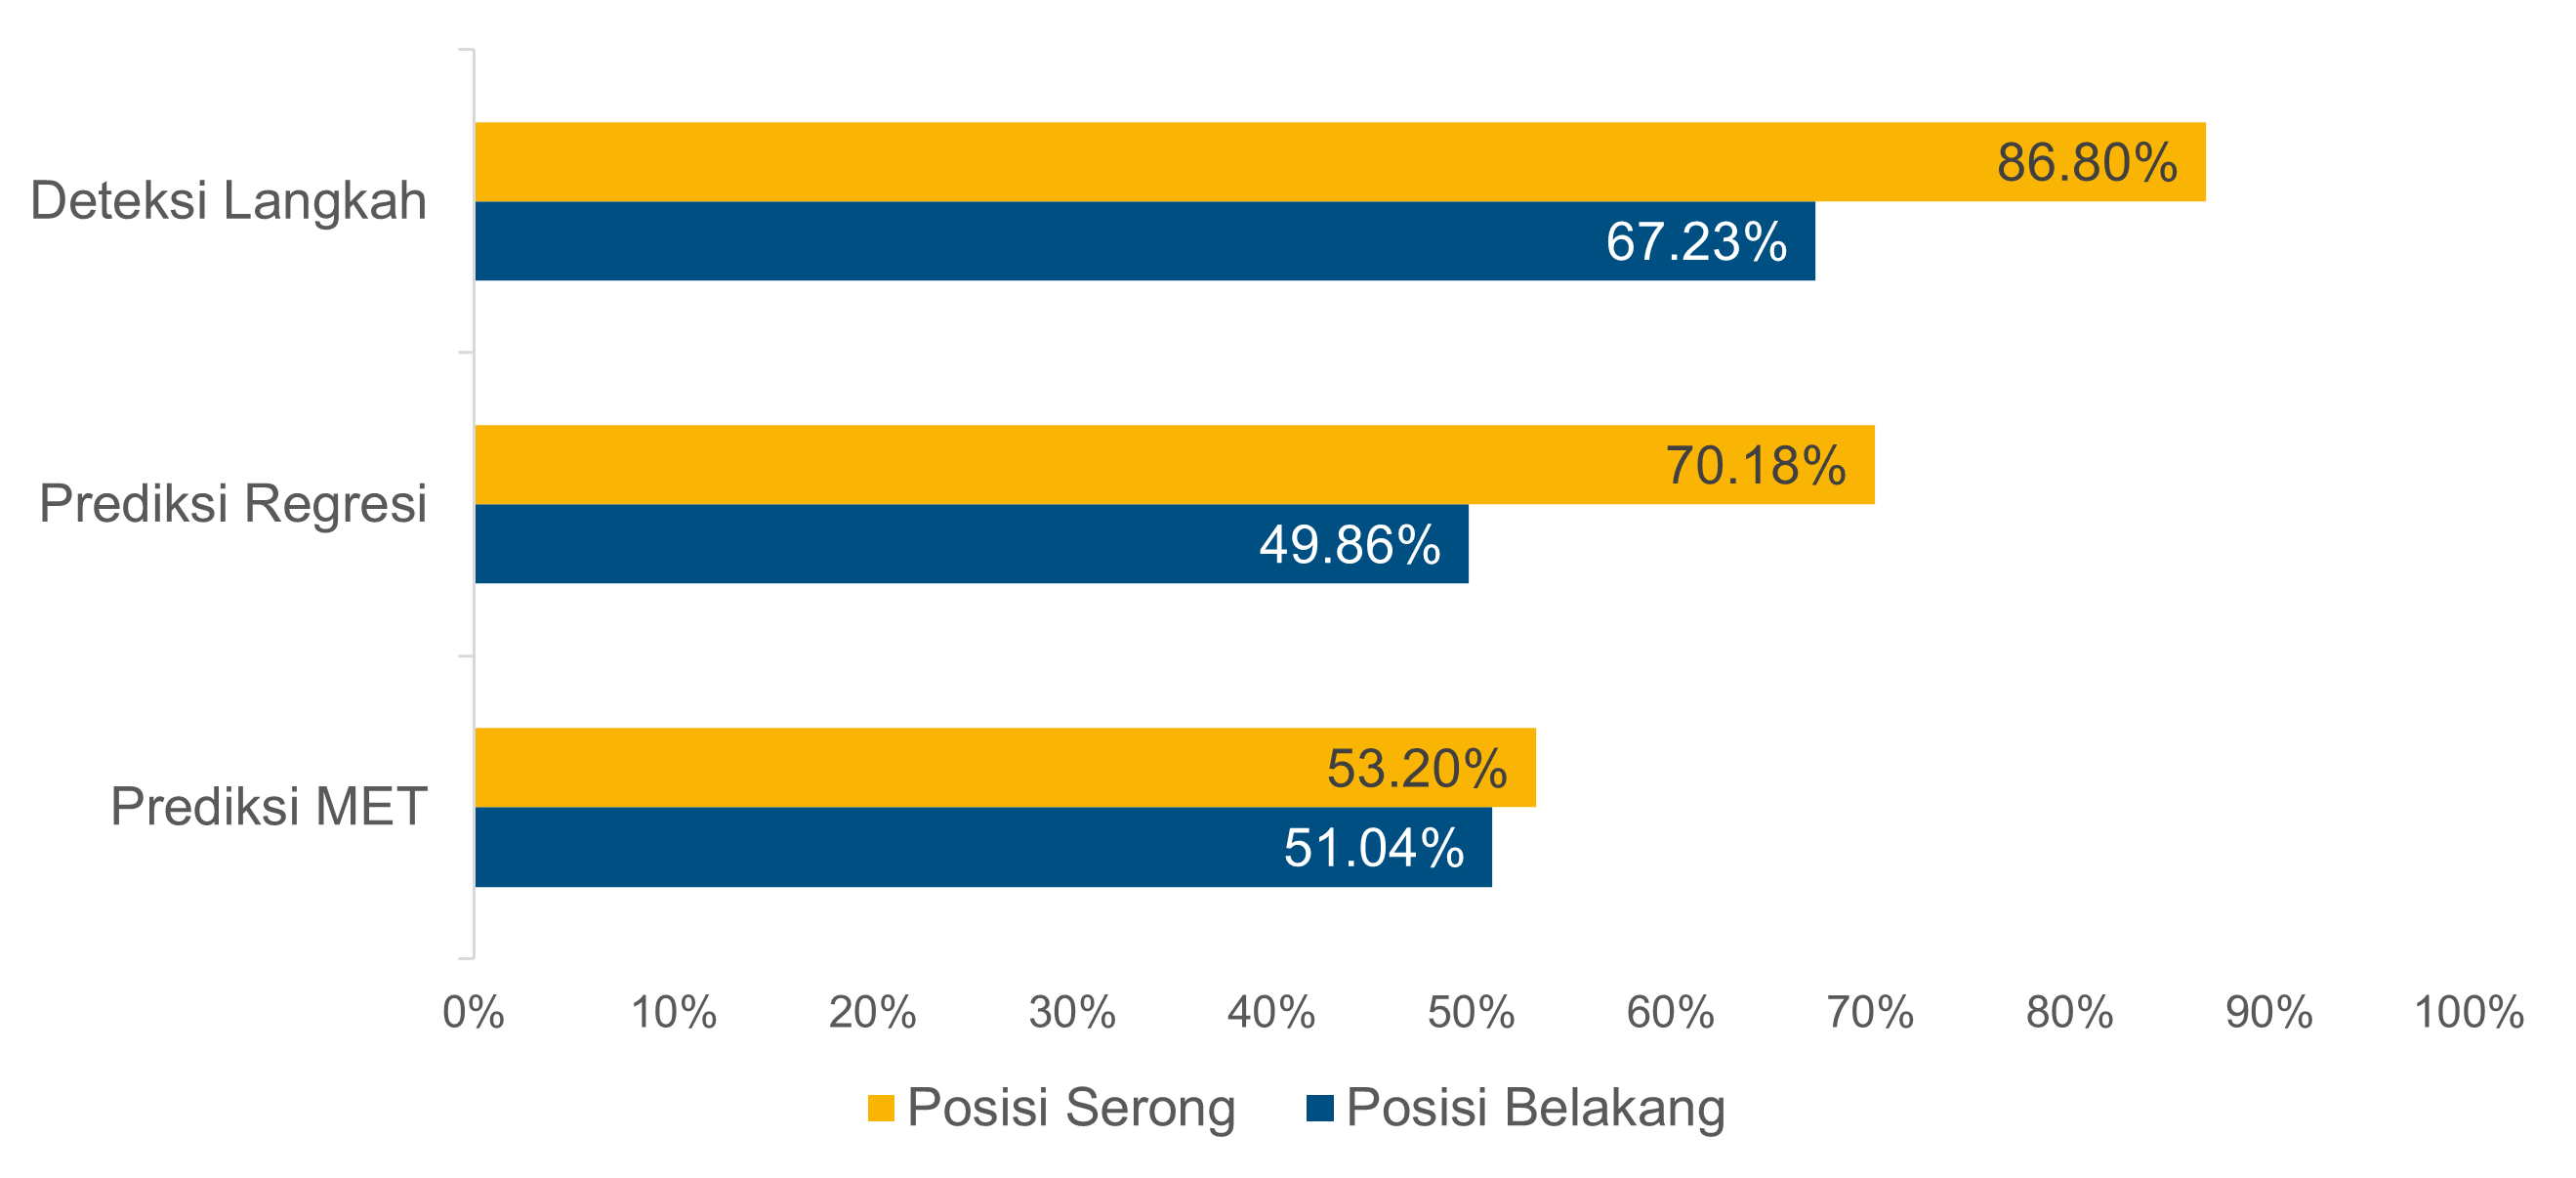
\includegraphics[scale=0.7]{gambar/diagram_posisi.png}
  \caption{Diagram perbandingan performa berdasarkan posisi kamera}
  \label{fig:DiagramPosisi}
\end{figure}

\section{Pengujian Performa Berdasarkan Intensitas Cahaya}
\label{sec:PengujianIntensitas}

Pada pengujian ini dilakukan deteksi dan prediksi kalori dengan menggunakan skenario berdasarkan intensitas cahaya yang berbeda-beda. Skenario pertama yang dilakukan adalah pengujian pada intensitas cahaya rendah, cahaya rendah yang digunakan berdasarkan pada nilai rata-rata kecerahan yang rendah pada setiap frame yang digunakan pada video percobaan. Skenario kedua yang dilakukan adalah pengujian pada intensitas cahaya tinggi, cahaya tinggi yang digunakan berdasarkan pada nilai rata-rata kecerahan yang tinggi pada setiap frame yang digunakan pada video percobaan. Video pengujian yang digunakan dengan banyak percobaan sebanyak 9 kali dengan menggunakan variasi kecepatan dan hasil kalori yang didapatkan. Variasi kecepatan yang digunakan adalah 3 km/jam, 9 km/jam dan 12 km/jam. Kemudian variasi hasil kalori yang didapatkan adalah 10 dan 20 kcal. 

\subsection{Pengujian Pada Intensitas Cahaya Rendah}
\label{subsec:PengujianIntensitasRendah}

Pengujian dilakukan dengan melakukan pengujian performa sistem pada intensitas cahaya rendah. Contoh cuplikan gambar yang memperlihatkan kondisi intensitas cahaya rendah dapat dilihat pada Gambar \ref{fig:PengujianIntensitasRendah}. Data percobaan yang digunakan dalam pengujian ini dilakukan proses deteksi dengan sistem yang dibuat untuk dapat melakukan proses estimasi dan deteksi langkah maupun waktu. Proses deteksi yang dilakukan pada data percobaan dapat dilihaat pada Gambar \ref{fig:PengujianIntensitasRendah2}. Pengujian dilanjutkan dengan melakukan proses prediksi dari hasil deteksi.

\begin{figure}[H]
  \centering
  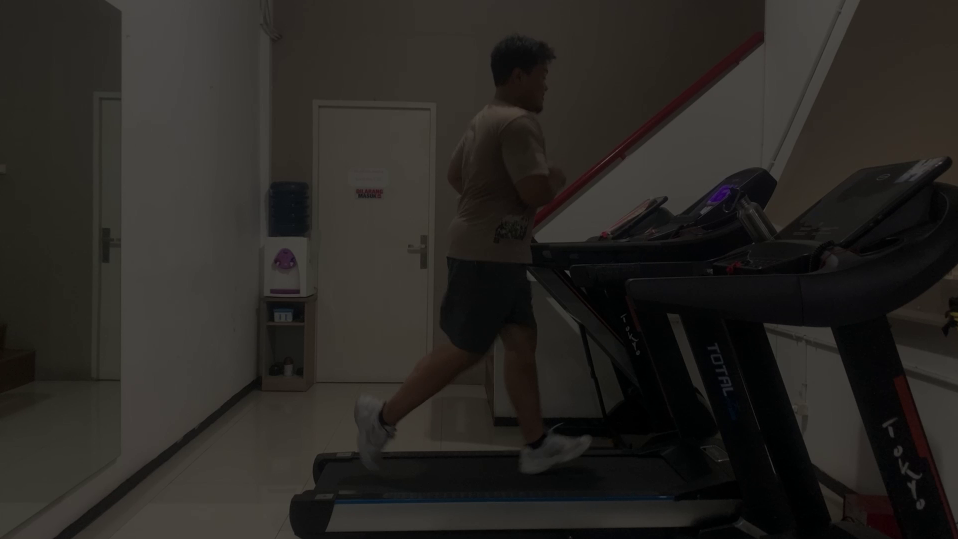
\includegraphics[scale=0.5]{gambar/cahaya_rendah.png}
  \caption{Pengujian pada intensitas cahaya rendah}
  \label{fig:PengujianIntensitasRendah}
\end{figure}

\begin{figure}[H]
  \centering
  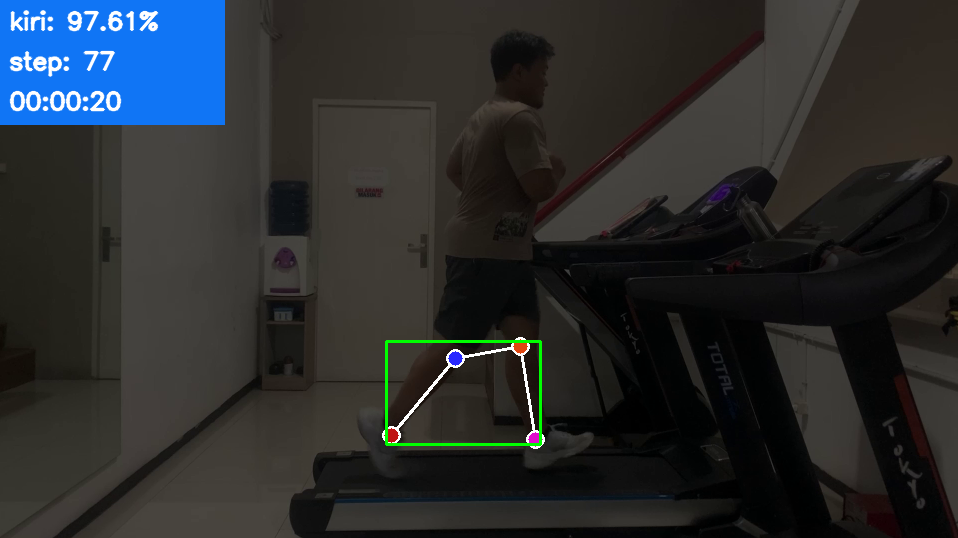
\includegraphics[scale=0.5]{gambar/cahaya_rendah2.png}
  \caption{Hasil deteksi pengujian pada intensitas cahaya rendah}
  \label{fig:PengujianIntensitasRendah2}
\end{figure}

Pengujian dilakukan setelah didapatkan data hasil deteksi yang telah didapat dan juga data sebenarnya berdasarkan hasil perhitungan yang dilakukan terhadap data video. Dengan data video sebagai banyaknya percobaan dilakukan analisa terkait perbandingan hasil yang didapat antara data hasil deteksi dan data perhitungan sebenarnya. Data langkah merupakan data sebagai data sebenarnya atau \emph{actual score} dengan melakukan perhitungan pada data video dan data deteksi langkah sebagai data hasil deteksi langkah yang didapatkan berdasarkan proses deteksi pada sistem. Perbandingan hasil deteksi dengan data sebenarnya dicantumkan pada data eror dan dilakukan persentase berdasarkan data sebenarnya. Hasil persentase eror mendapatkan hasil persentase akurasi yang juga didapatkan berdasarkan persentase eror. Hasil analisa yang didapat dengan melakukan analisa pengujian hasil deteksi didapatkan hasil akurasi rata-rata sebesar 90,69\% dengan hasil eror rata-rata sebesar 9,31\%. Tabel \ref{tb:PengujianIntensitasRendahAnalisaDeteksi} menunjukkan hasil pengujian dari setiap percobaan yang dilakukan analisa pengujian terhadap hasil deteksi.

\begin{longtable}{|c|c|c|c|c|c|}
  \caption{Hasil Deteksi Pengujian Pada Intensitas Cahaya Rendah}
  \label{tb:PengujianIntensitasRendahAnalisaDeteksi}                                   \\
  \hline
  \rowcolor[HTML]{C0C0C0}
  \textbf{Percobaan} & \textbf{Langkah} & \textbf{Deteksi Langkah} & \textbf{Error} & \textbf{Eror\%} & \textbf{Akurasi\%} \\
  \hline
  1   & 274   & 274 & 0    & 0\%       & 100\%   \\
  \hline
  2   & 260   & 260 & 0    & 0\%       & 100\%   \\
  \hline
  3   & 276   & 254 & 22   & 7,97\%    & 92,03\%     \\
  \hline
  4   & 321   & 304 & 17   & 5,30\%    & 94,70\%   \\
  \hline
  5   & 309   & 311 & 2    & 0,65\%    & 99,35\%   \\
  \hline
  6   & 317   & 268 & 49   & 15,46\%   & 84,54\%   \\
  \hline
  7   & 276   & 228 & 48   & 17,39\%   & 82,61\%   \\
  \hline
  8   & 259   & 258 & 1    & 0,39\%    & 99,61\%   \\
  \hline
  9   & 292   & 185 & 107  & 36,64\%   & 63,36\%   \\
  \hline

  \multicolumn{4}{|c|}{\textbf{Rata-rata}} & 9,31\% & 90,69\% \\
  \hline
\end{longtable}

Pada pengujian prediksi kalori dilakukan berdasarkan hasil deteksi yang didapat. Hasil deteksi berupa banyaknya langkah, jarak dan waktu tempuh dari data video yang digunakan. Data hasil deteksi akan diilakukan untuk proses prediksi kalori dengan menggunakan model regresi linear yang sudah didapatkan dan menghasilkan data pada prediksi kalori. Analisa pengujian hasil prediksi kalori dilakukan dengan melakukan perbandingan data prediksi kalori dari sistem yang digunakan dengan data kalori treadmill sebagai data sebenarnya atau data \emph{actual score}. Perbandingan hasil prediksi kalori dengan kalori treadmill didapatkan data eror yang kemudian dilakukan perhitungan persentase berdasarkan data sebenarnya pada data kalori treadmill. Proses analisa pengujian dilakukan terhadap seluruh data video pada data percobaan. Hasil analisa yang didapat dengan melakukan analisa pengujian prediksi kalori didapatkan hasil akurasi rata-rata sebesar 73,68\% dengan hasil eror rata-rata sebesar 26,32\%. Tabel \ref{tb:PengujianIntensitasRendahAnalisaPrediksiRegresi} menunjukkan hasil analisa pengujian dari setiap percobaan yang dilakukan analisa prediksi kalori dengan regresi linear.

\begin{longtable}{|c|c|c|c|c|c|c|c|}
  \caption{Hasil Prediksi Pengujian Pada Intensitas Cahaya Rendah dengan Regresi Linear}
  \label{tb:PengujianIntensitasRendahAnalisaPrediksiRegresi}                                   \\
  \hline
  \rowcolor[HTML]{C0C0C0}
  & & & & \textbf{Kalori} & \textbf{Prediksi} & & \\
  \rowcolor[HTML]{C0C0C0}
  \multirow{-2}{*}{\textbf{Percobaan}} & \multirow{-2}{*}{\textbf{Langkah}} & \multirow{-2}{*}{\textbf{Jarak}} & \multirow{-2}{*}{\textbf{Waktu}} & \textbf{Treadmill} & \textbf{Kalori} & \multirow{-2}{*}{\textbf{Eror\%}} & \multirow{-2}{*}{\textbf{Akurasi\%}} \\
  
  \hline
  1   & 274   & 175,936    & 2:49    & 10    & 12,267   & 23,67\%    & 77,33\%   \\
  \hline  
  2   & 260   & 177,780    & 2:49    & 10    & 12,397   & 23,97\%    & 76,03\%  \\
  \hline
  3   & 254   & 176,568    & 2:49    & 10    & 12,312   & 23,12\%    & 76,88\%   \\
  \hline
  4   & 304   & 263,156    & 2:01    & 20    & 18,422   & 7,89\%     & 92,11\%  \\
  \hline
  5   & 311   & 291,916    & 2:02    & 20    & 20,447   & 2,23\%     & 97,77\%    \\
  \hline
  6   & 268   & 143,707    & 2:02    & 20    & 10,013   & 49,93\%    & 50,07\%   \\
  \hline
  7   & 228   & 169,023    & 1:39    & 20    & 11,802   & 40,99\%    & 59,01\%   \\
  \hline
  8   & 258   & 269,480    & 1:40    & 20    & 18,874   & 5,63\%     & 94,37\%   \\
  \hline
  9   & 185   & 113,831    & 1:45    & 20    & 7,915    & 60,42\%    & 39,58\%   \\
  \hline

  \multicolumn{6}{|c|}{\textbf{Rata-rata}} & 26,32\% & 73,68\% \\
  \hline
\end{longtable}

Pada pengujian prediksi kalori dilakukan berdasarkan hasil deteksi yang didapat. Hasil deteksi berupa kecepatan, MET dan waktu tempuh dari data video yang digunakan. Data hasil deteksi akan diilakukan untuk proses prediksi kalori dengan menggunakan perhitungan rumus berdasarkan MET yang sudah didapatkan dan menghasilkan data pada prediksi kalori. Analisa pengujian hasil prediksi kalori dilakukan dengan melakukan perbandingan data prediksi kalori dari sistem yang digunakan dengan data kalori treadmill sebagai data sebenarnya atau data \emph{actual score}. Perbandingan hasil prediksi kalori dengan kalori treadmill didapatkan data eror yang kemudian dilakukan perhitungan persentase berdasarkan data sebenarnya pada data kalori treadmill. Proses analisa pengujian dilakukan terhadap seluruh data video pada data percobaan. Hasil analisa yang didapat dengan melakukan analisa pengujian prediksi kalori didapatkan hasil akurasi rata-rata sebesar 58,08\% dengan hasil eror rata-rata sebesar 41,92\%. Tabel \ref{tb:PengujianIntensitasRendahAnalisaPrediksiPerhitungan} menunjukkan hasil analisa pengujian dari prediksi kalori dengan perhitungan rumus.

\begin{longtable}{|c|c|c|c|c|c|c|c|}
  \caption{Hasil Prediksi Pengujian Pada Intensitas Cahaya Rendah dengan Perhitungan Rumus}
  \label{tb:PengujianIntensitasRendahAnalisaPrediksiPerhitungan}                                   \\
  \hline
  \rowcolor[HTML]{C0C0C0}
  & & & & \textbf{Kalori} & \textbf{Prediksi} & & \\
  \rowcolor[HTML]{C0C0C0}
  \multirow{-2}{*}{\textbf{Percobaan}} & \multirow{-2}{*}{\textbf{Kecepatan}} & \multirow{-2}{*}{\textbf{MET}} & \multirow{-2}{*}{\textbf{Waktu}} & \textbf{Treadmill} & \textbf{Kalori} & \multirow{-2}{*}{\textbf{Eror\%}} & \multirow{-2}{*}{\textbf{Akurasi\%}} \\
  \hline
  1   & 3,572   & 2,178    & 2:50    & 10   & 6,979    & 30,21\%     & 69,79\%   \\
  \hline
  2   & 3,820   & 1,192    & 1:35    & 10   & 3,819    & 61,81\%     & 38,19\%   \\
  \hline
  3   & 3,880   & 0,966    & 2:02    & 10   & 3,095    & 69,05\%     & 30,95\%   \\
  \hline
  4   & 7,987   & 8,337    & 1:41    & 20   & 19,125   & 4,38\%      & 95,62\%   \\
  \hline
  5   & 8,735   & 9,114    & 2:03    & 20   & 21,079   & 5,40\%      & 94,60\%   \\
  \hline
  6   & 3,653   & 1,852    & 1:21    & 20   & 4,389    & 78,05\%     & 21,95\%   \\
  \hline
  7   & 6,319   & 5,818    & 1:39    & 20   & 10,920   & 45,40\%     & 54,60\%   \\
  \hline
  8   & 9,869   & 10,024   & 1:37    & 20   & 19,004   & 4,98\%      & 95,05\%   \\
  \hline
  9   & 3,574   & 2,171    & 1:45    & 20   & 4,403    & 77,98\%     & 22,02\%   \\
  \hline

  \multicolumn{6}{|c|}{\textbf{Rata-rata}} & 41,92\% & 58,08\%  \\
  \hline
\end{longtable}


\subsection{Pengujian Pada Intensitas Cahaya Tinggi}
\label{subsec:PengujianIntensitasTinggi}

Pengujian dilakukan dengan melakukan pengujian performa sistem pada intensitas cahaya tinggi. Contoh cuplikan gambar yang memperlihatkan kondisi intensitas cahaya tinggi dapat dilihat pada Gambar \ref{fig:PengujianIntensitasTinggi}. Data percobaan yang digunakan dalam pengujian ini dilakukan proses deteksi dengan sistem yang dibuat untuk dapat melakukan proses estimasi dan deteksi langkah maupun waktu. Proses deteksi yang dilakukan pada data percobaan dapat dilihaat pada Gambar \ref{fig:PengujianIntensitasTinggi2}. Pengujian dilanjutkan dengan melakukan proses prediksi dari hasil deteksi.

\begin{figure}[H]
  \centering
  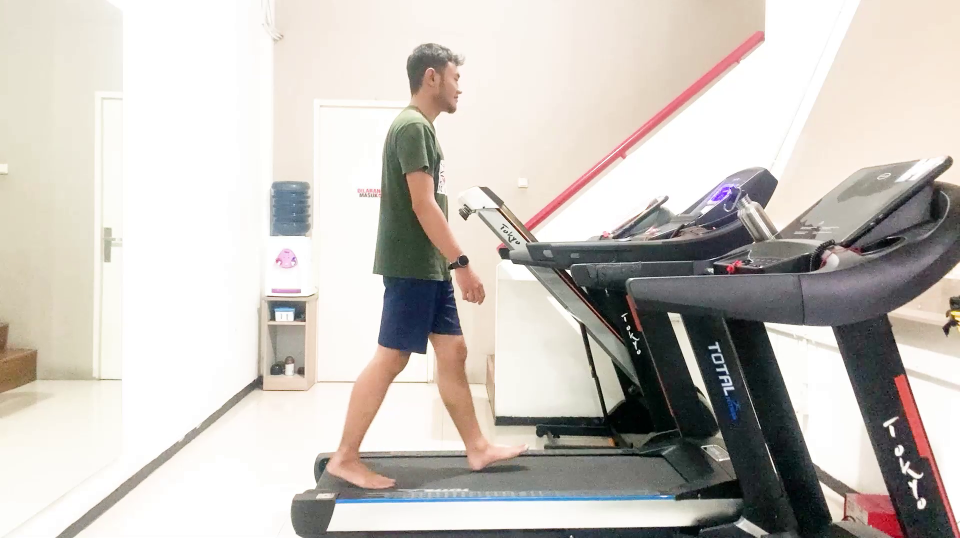
\includegraphics[scale=0.5]{gambar/cahaya_tinggi.png}
  \caption{Pengujian pada intensitas cahaya tinggi}
  \label{fig:PengujianIntensitasTinggi}
\end{figure}

\begin{figure}[H]
  \centering
  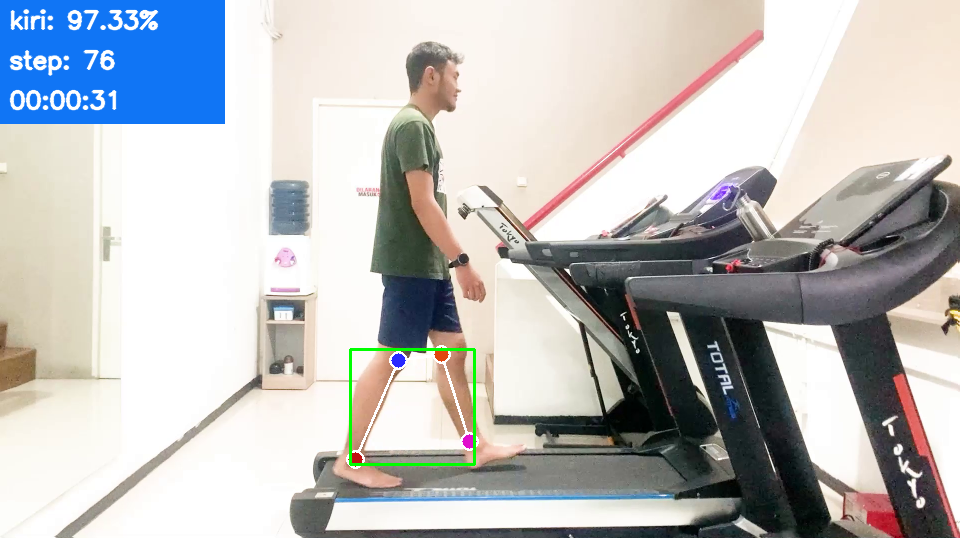
\includegraphics[scale=0.5]{gambar/cahaya_tinggi2.png}
  \caption{Hasil deteksi pengujian pada intensitas cahaya tinggi}
  \label{fig:PengujianIntensitasTinggi2}
\end{figure}

Pengujian dilakukan setelah didapatkan data hasil deteksi yang telah didapat dan juga data sebenarnya berdasarkan hasil perhitungan yang dilakukan terhadap data video. Dengan data video sebagai banyaknya percobaan dilakukan analisa terkait perbandingan hasil yang didapat antara data hasil deteksi dan data perhitungan sebenarnya. Data langkah merupakan data sebagai data sebenarnya atau \emph{actual score} dengan melakukan perhitungan pada data video dan data deteksi langkah sebagai data hasil deteksi langkah yang didapatkan berdasarkan proses deteksi pada sistem. Perbandingan hasil deteksi dengan data sebenarnya dicantumkan pada data eror dan dilakukan persentase berdasarkan data sebenarnya. Hasil persentase eror mendapatkan hasil persentase akurasi yang juga didapatkan berdasarkan persentase eror. Hasil analisa yang didapat dengan melakukan analisa pengujian hasil deteksi didapatkan hasil akurasi rata-rata sebesar 95,54\% dengan hasil eror rata-rata sebesar 4,46\%. Tabel \ref{tb:PengujianIntensitasTinggiAnalisaDeteksi} menunjukkan hasil pengujian dari setiap percobaan yang dilakukan analisa pengujian terhadap hasil deteksi.

\begin{longtable}{|c|c|c|c|c|c|}
  \caption{Hasil Deteksi Pengujian Pada Intensitas Cahaya Tinggi}
  \label{tb:PengujianIntensitasTinggiAnalisaDeteksi}                                   \\
  \hline
  \rowcolor[HTML]{C0C0C0}
  \textbf{Percobaan} & \textbf{Langkah} & \textbf{Deteksi Langkah} & \textbf{Eror} & \textbf{Eror\%} & \textbf{Akurasi\%} \\
  \hline
  1   & 274   & 274 & 0    & 0\%        & 100\%   \\
  \hline
  2   & 260   & 256 & 4    & 1,54\%     & 99,46\%   \\
  \hline
  3   & 276   & 268 & 8    & 2,90\%     & 97,10\%     \\
  \hline
  4   & 321   & 334 & 13   & 4,05\%     & 95,95\%   \\
  \hline
  5   & 309   & 312 & 3    & 0,97\%     & 99,03\%   \\
  \hline
  6   & 317   & 296 & 21   & 6,62\%     & 93,38\%   \\
  \hline
  7   & 276   & 240 & 36   & 13,04\%    & 86,96\%   \\
  \hline
  8   & 259   & 260 & 1    & 0,39\%     & 99,61\%   \\
  \hline
  9   & 292   & 261 & 31   & 10,62\%    & 89,38\%   \\
  \hline
  

  \multicolumn{4}{|c|}{\textbf{Rata-rata}} & 4,46\% & 95,54\% \\
  \hline
\end{longtable}

Pada pengujian prediksi kalori dilakukan berdasarkan hasil deteksi yang didapat. Hasil deteksi berupa banyaknya langkah, jarak dan waktu tempuh dari data video yang digunakan. Data hasil deteksi akan diilakukan untuk proses prediksi kalori dengan menggunakan model regresi linear yang sudah didapatkan dan menghasilkan data pada prediksi kalori. Analisa pengujian hasil prediksi kalori dilakukan dengan melakukan perbandingan data prediksi kalori dari sistem yang digunakan dengan data kalori treadmill sebagai data sebenarnya atau data \emph{actual score}. Perbandingan hasil prediksi kalori dengan kalori treadmill didapatkan data eror yang kemudian dilakukan perhitungan persentase berdasarkan data sebenarnya pada data kalori treadmill. Proses analisa pengujian dilakukan terhadap seluruh data video pada data percobaan. Hasil analisa yang didapat dengan melakukan analisa pengujian prediksi kalori didapatkan hasil akurasi rata-rata sebesar 73,61\% dengan hasil eror rata-rata sebesar 26,39\%. Tabel \ref{tb:PengujianIntensitasTinggiAnalisaPrediksiRegresi} menunjukkan hasil analisa pengujian dari setiap percobaan yang dilakukan analisa prediksi kalori dengan regresi linear.

\begin{longtable}{|c|c|c|c|c|c|c|c|}
  \caption{Hasil Prediksi Pengujian Pada Intensitas Cahaya Tinggi dengan Regresi Linear}
  \label{tb:PengujianIntensitasTinggiAnalisaPrediksiRegresi}                                   \\
  \hline
  \rowcolor[HTML]{C0C0C0}
  & & & & \textbf{Kalori} & \textbf{Prediksi} & & \\
  \rowcolor[HTML]{C0C0C0}
  \multirow{-2}{*}{\textbf{Percobaan}} & \multirow{-2}{*}{\textbf{Langkah}} & \multirow{-2}{*}{\textbf{Jarak}} & \multirow{-2}{*}{\textbf{Waktu}} & \textbf{Treadmill} & \textbf{Kalori} & \multirow{-2}{*}{\textbf{Eror\%}} & \multirow{-2}{*}{\textbf{Akurasi\%}} \\
  
  \hline
  1   & 274   & 175,936    & 2:49    & 10    & 12,267   & 22,67\%      & 77,33\%   \\
  \hline  
  2   & 256   & 177,101    & 2:49    & 10    & 12,349   & 23,49\%      & 76,51\%  \\
  \hline
  3   & 268   & 177,545    & 2:49    & 10    & 12,381   & 23,81\%      & 76,19\%   \\
  \hline
  4   & 334   & 533,158    & 2:01    & 20    & 37,430   & 87,15\%      & 12,85\%  \\
  \hline
  5   & 312   & 298,637    & 2:02    & 20    & 20,920   & 4,60\%       & 95,40\%    \\
  \hline
  6   & 296   & 212,781    & 2:02    & 20    & 14,876   & 25,62\%      & 74,38\%   \\
  \hline
  7   & 240   & 202,035    & 1:39    & 20    & 14,126   & 29,37\%      & 70,63\%   \\
  \hline
  8   & 260   & 280,461    & 1:40    & 20    & 19,647   & 1,76\%       & 98,24\%   \\
  \hline
  9   & 261   & 231,528    & 1:45    & 20    & 16,201   & 18,99\%      & 81,01\%   \\
  \hline

  \multicolumn{6}{|c|}{\textbf{Rata-rata}} & 26,39\% & 73,61\% \\
  \hline
\end{longtable}

Pada pengujian prediksi kalori dilakukan berdasarkan hasil deteksi yang didapat. Hasil deteksi berupa kecepatan, MET dan waktu tempuh dari data video yang digunakan. Data hasil deteksi akan diilakukan untuk proses prediksi kalori dengan menggunakan perhitungan rumus berdasarkan MET yang sudah didapatkan dan menghasilkan data pada prediksi kalori. Analisa pengujian hasil prediksi kalori dilakukan dengan melakukan perbandingan data prediksi kalori dari sistem yang digunakan dengan data kalori treadmill sebagai data sebenarnya atau data \emph{actual score}. Perbandingan hasil prediksi kalori dengan kalori treadmill didapatkan data eror yang kemudian dilakukan perhitungan persentase berdasarkan data sebenarnya pada data kalori treadmill. Proses analisa pengujian dilakukan terhadap seluruh data video pada data percobaan. Hasil analisa yang didapat dengan melakukan analisa pengujian prediksi kalori didapatkan hasil akurasi rata-rata sebesar 68,92\% dengan hasil eror rata-rata sebesar 31,08\%. Tabel \ref{tb:PengujianIntensitasTinggiAnalisaPrediksiPerhitungan} menunjukkan hasil analisa pengujian dari prediksi kalori dengan perhitungan rumus.

\begin{longtable}{|c|c|c|c|c|c|c|c|}
  \caption{Hasil Prediksi Pengujian Pada Intensitas Cahaya Tinggi dengan Perhitungan Rumus}
  \label{tb:PengujianIntensitasTinggiAnalisaPrediksiPerhitungan}                                   \\
  \hline
  \rowcolor[HTML]{C0C0C0}
  & & & & \textbf{Kalori} & \textbf{Prediksi} & & \\
  \rowcolor[HTML]{C0C0C0}
  \multirow{-2}{*}{\textbf{Percobaan}} & \multirow{-2}{*}{\textbf{Kecepatan}} & \multirow{-2}{*}{\textbf{MET}} & \multirow{-2}{*}{\textbf{Waktu}} & \textbf{Treadmill} & \textbf{Kalori} & \multirow{-2}{*}{\textbf{Eror\%}} & \multirow{-2}{*}{\textbf{Akurasi\%}} \\
  \hline
  1   & 3,572   & 2,178    & 2:49    & 10   & 6,979   & 30,21\%     & 69,79\%   \\
  \hline
  2   & 3,862   & 1,029    & 2:49    & 10   & 3,296   & 67,04\%     & 32,96\%   \\
  \hline
  3   & 3,697   & 1,675    & 2:49    & 20   & 5,367   & 46,33\%     & 53,67\%   \\
  \hline
  4   & 15,114  & 13,453   & 2:01    & 20   & 30,862  & 54,31\%     & 45,69\%   \\
  \hline
  5   & 8,923   & 9,283    & 2:02    & 20   & 21,471  & 7,36\%      & 92,64\%   \\
  \hline
  6   & 6,427   & 6,023    & 2:02    & 20   & 13,930  & 30,35\%     & 69,65\%   \\
  \hline
  7   & 7,589   & 7,846    & 1:39    & 20   & 14,726  & 26,37\%     & 73,63\%   \\
  \hline
  8   & 10,234  & 10,270   & 1:40    & 20   & 19,470  & 2,65\%      & 97,35\%   \\
  \hline
  9   & 8,160   & 8,533    & 1:45    & 20   & 16,985  & 15,07\%     & 84,93\%   \\
  \hline

  \multicolumn{6}{|c|}{\textbf{Rata-rata}} & 31,08\% & 68,92\%  \\
  \hline
\end{longtable}

Berdasarkan pengujian yang telah dilakukan terhadap hasil performa deteksi langkah, prediksi kalori dengan regresi dan prediksi kalori dengan perhitungan rumus didapatkan hasil performa dalam nilai akurasi rata-rata dan eror rata-rata dari setiap pengujian. Pada pengujian deteksi langkah didapatkan akurasi rata-rata lebih baik pada intensitas cahaya tinggi dengan nilai akurasi rata-rata sebesar 95,54\% sedangkan pada intensitas cahaya rendah didapat nilai akurasi rata-rata sebesar 90,69\%. Pada pengujian prediksi kalori dengan regresi didapatkan akurasi rata-rata lebih baik pada intensitas cahaya rendah dengan nilai akurasi rata-rata sebesar 73,68\% sedangkan pada intensitas cahaya tinggi didapat nilai akurasi rata-rata sebesar 73,61\%. Pada pengujian prediksi kalori dengan perhitungan rumus didapatkan akurasi rata-rata lebih baik pada intensitas cahaya tinggi cm dengan nilai akurasi rata-rata sebesar 68,92\% sedangkan pada intensitas cahaya rendah didapat nilai akurasi rata-rata sebesar 58,08\%. Gambar \ref{fig:DiagramPosisi} menunjukkan diagram perbandingan performa pengujian dengan nilai akurasi rata-rata berdasarkan intensitas cahaya.

\begin{figure}[H]
  \centering
  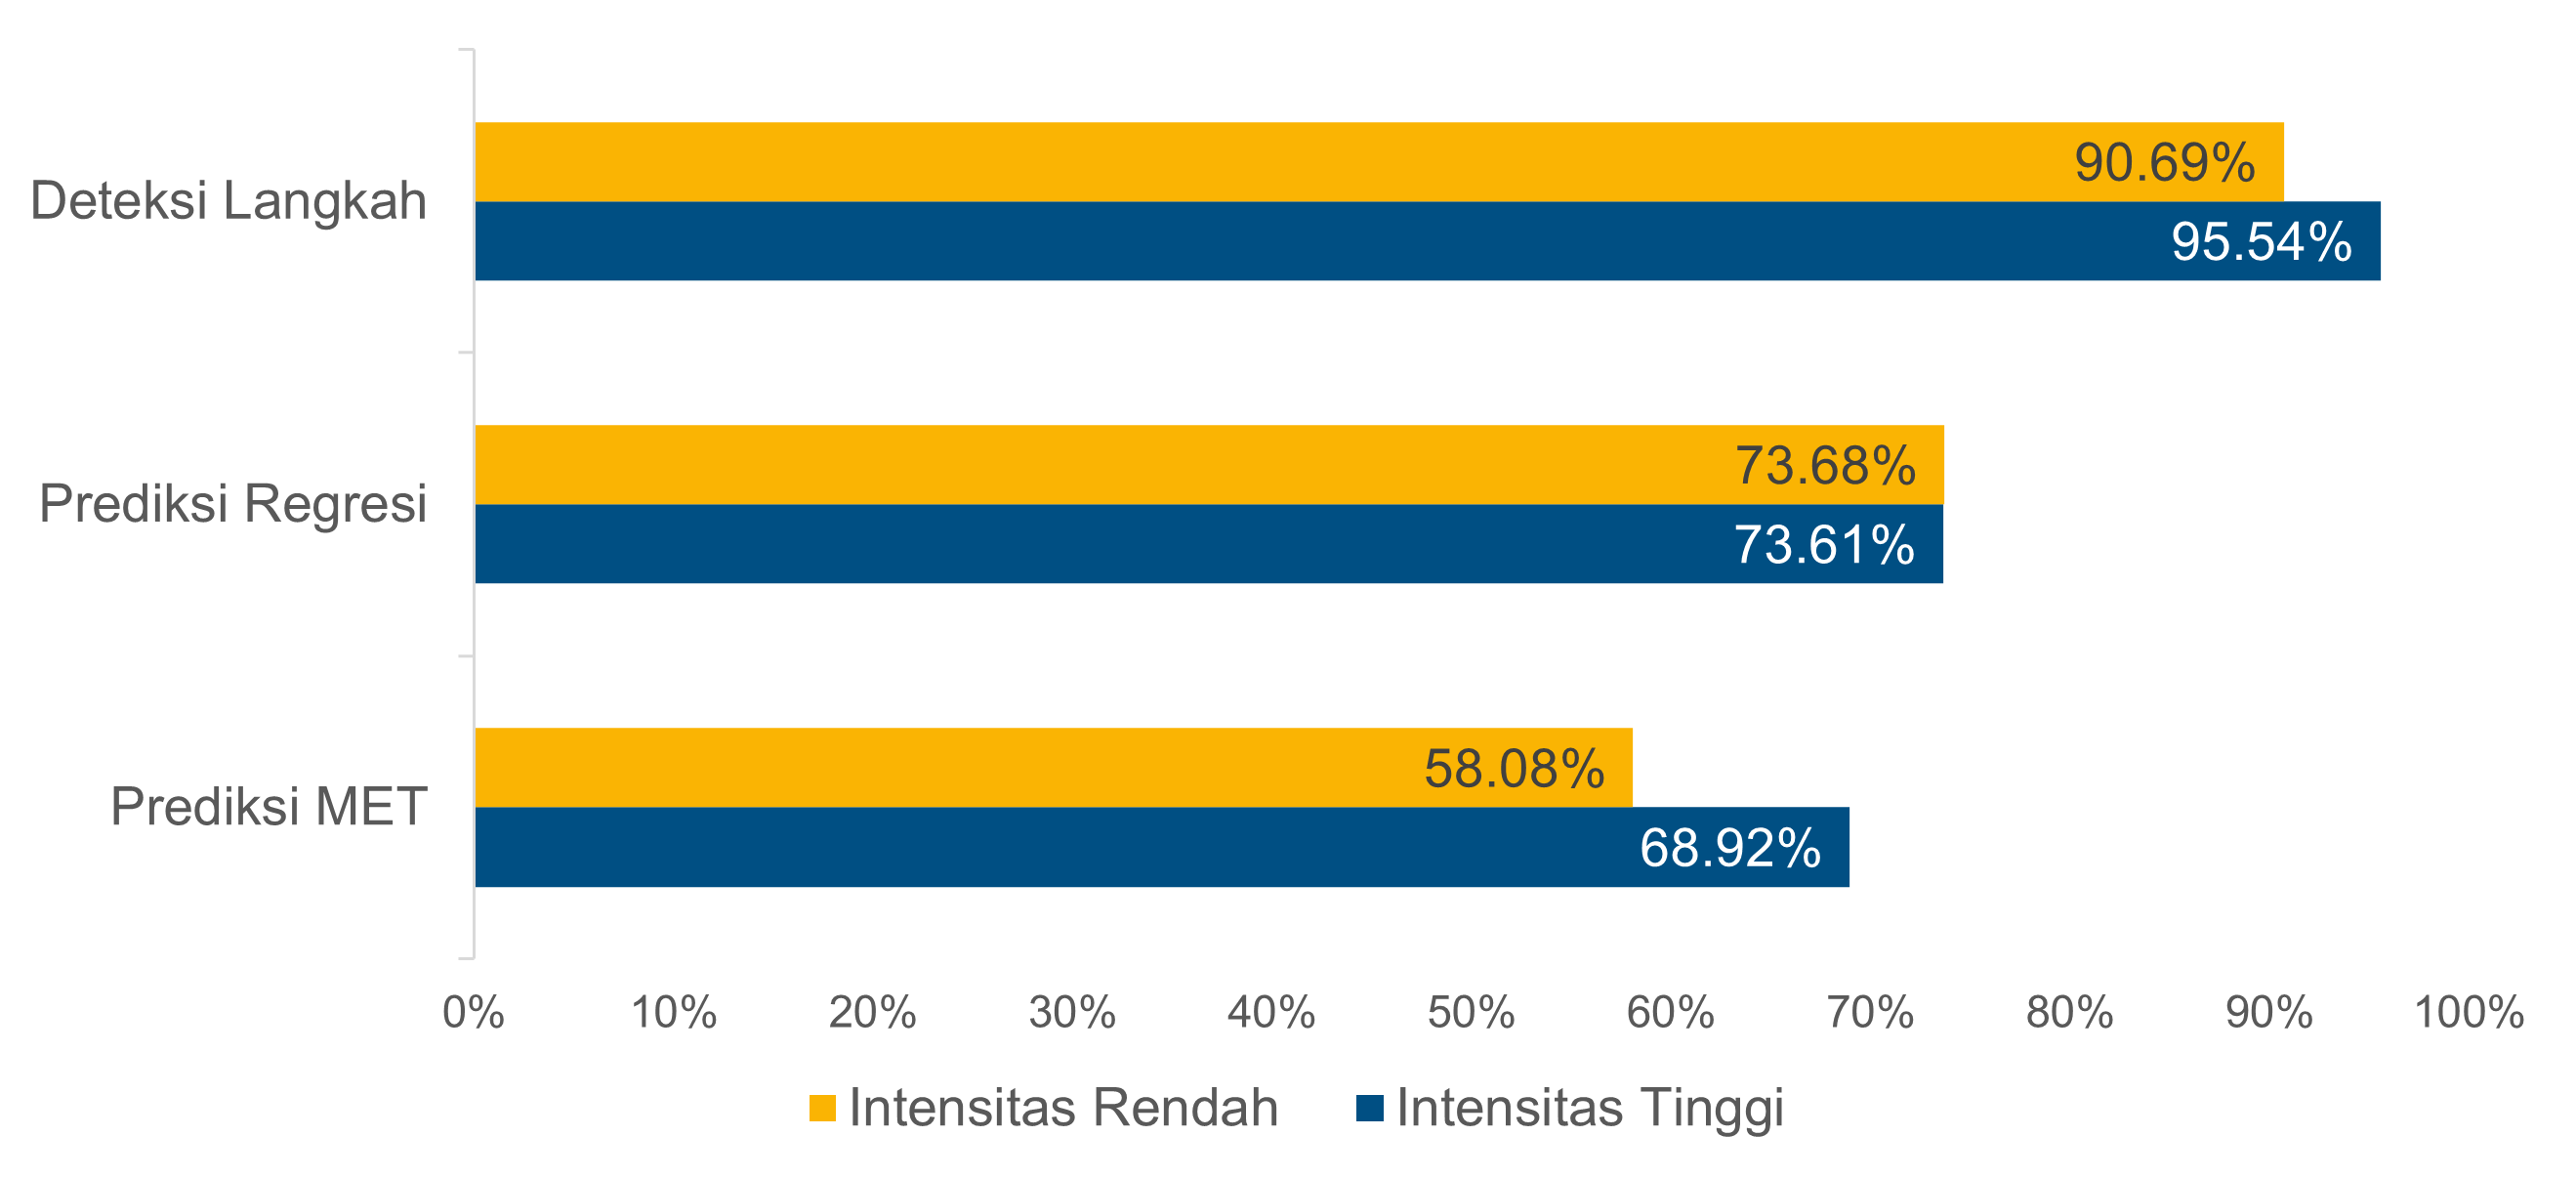
\includegraphics[scale=0.7]{gambar/diagram_cahaya.png}
  \caption{Diagram perbandingan performa berdasarkan intensitas cahaya}
  \label{fig:DiagramPosisi}
\end{figure}

\section{Pengujian Sistem secara \emph{Real Time}}
\label{sec:PengujianRealTime}

Pengujian dilakukan dengan melakukan pengujian sistem secara \emph{real Time} dengan melakukan proses sistem secara langsung pada objek yang dideteksi. Proses pengujian dilakukan dengan mengambil data video yang bersumber pada kamera yang akan langsung diproses pada perangkat yang digunakan untuk proses sistem. Data video yang digunakan akan digunakan sebagai data video percobaan dan data pengujian secara bersamaan. Percobaan pada pengujian yang dilakukan sebanyak 6 kali dengan menggunakan variasi kecepatan dan hasil kalori yang didapatkan. Variasi kecepatan yang digunakan adalah 4 km/jam dan 12 km/jam. Kemudian variasi hasil kalori yang didapatkan adalah 5 dan 20 kcal.

Data percobaan yang digunakan dalam pengujian ini dilakukan proses deteksi dengan sistem yang dibuat untuk dapat melakukan proses estimasi dan deteksi langkah maupun waktu. Proses deteksi yang dilakukan pada data percobaan dapat dilihaat pada Gambar \ref{fig:PengujianRealTime2}. Pengujian dilanjutkan dengan melakukan proses prediksi dari hasil deteksi.

\begin{figure}[H]
  \centering
  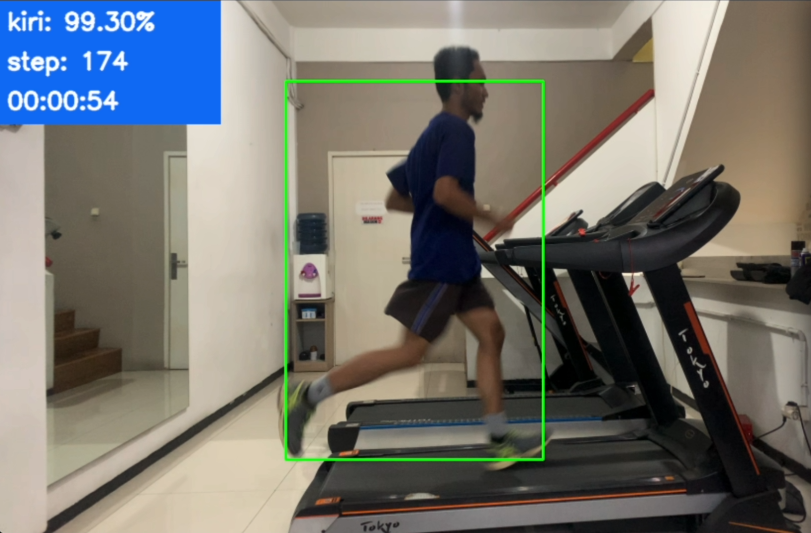
\includegraphics[scale=0.5]{gambar/realtimedeteksi.png}
  \caption{Hasil deteksi pengujian secara \emph{real time}}
  \label{fig:PengujianRealTime2}
\end{figure}

Pengujian dilakukan setelah didapatkan data hasil deteksi yang telah didapat dan juga data sebenarnya berdasarkan hasil perhitungan yang dilakukan terhadap data video. Dengan data video sebagai banyaknya percobaan dilakukan analisa terkait perbandingan hasil yang didapat antara data hasil deteksi dan data perhitungan sebenarnya. Data langkah merupakan data sebagai data sebenarnya atau \emph{actual score} dengan melakukan perhitungan pada data video dan data deteksi langkah sebagai data hasil deteksi langkah yang didapatkan berdasarkan proses deteksi pada sistem. Perbandingan hasil deteksi dengan data sebenarnya dicantumkan pada data eror dan dilakukan persentase berdasarkan data sebenarnya. Hasil persentase eror mendapatkan hasil persentase akurasi yang juga didapatkan berdasarkan persentase eror. Hasil analisa yang didapat dengan melakukan analisa pengujian hasil deteksi didapatkan hasil akurasi rata-rata sebesar 81,35\% dengan hasil eror rata-rata sebesar 18,65\%. Tabel \ref{tb:PengujianRealTimeAnalisaDeteksi} menunjukkan hasil pengujian dari setiap percobaan yang dilakukan analisa pengujian terhadap hasil deteksi.

\begin{longtable}{|c|c|c|c|c|c|}
  \caption{Hasil Deteksi Pengujian Sistem secara \emph{Real Time}}
  \label{tb:PengujianRealTimeAnalisaDeteksi}                                   \\
  \hline
  \rowcolor[HTML]{C0C0C0}
  \textbf{Percobaan} & \textbf{Langkah} & \textbf{Deteksi Langkah} & \textbf{Eror} & \textbf{Eror\%} & \textbf{Akurasi\%} \\
  \hline
  1   & 105   & 101 & 4    & 3,81\%     & 96,19\%   \\
  \hline
  2   & 125   & 124 & 1    & 0,80\%     & 99,20\%   \\
  \hline
  3   & 117   & 104 & 13   & 11,11\%    & 88,89\%     \\
  \hline
  4   & 255   & 214 & 41   & 16,08\%    & 83,92\%   \\
  \hline
  5   & 269   & 230 & 39   & 14,50\%    & 85,50\%   \\
  \hline
  6   & 220   & 218 & 187  & 65,61\%    & 34,39\%   \\
  \hline

  \multicolumn{4}{|c|}{\textbf{Rata-rata}} & 18,65\% & 81,35\% \\
  \hline
\end{longtable}

Pada pengujian prediksi kalori dilakukan berdasarkan hasil deteksi yang didapat. Hasil deteksi berupa banyaknya langkah, jarak dan waktu tempuh dari data video yang digunakan. Data hasil deteksi akan diilakukan untuk proses prediksi kalori dengan menggunakan model regresi linear yang sudah didapatkan dan menghasilkan data pada prediksi kalori. Analisa pengujian hasil prediksi kalori dilakukan dengan melakukan perbandingan data prediksi kalori dari sistem yang digunakan dengan data kalori treadmill sebagai data sebenarnya atau data \emph{actual score}. Perbandingan hasil prediksi kalori dengan kalori treadmill didapatkan data eror yang kemudian dilakukan perhitungan persentase berdasarkan data sebenarnya pada data kalori treadmill. Proses analisa pengujian dilakukan terhadap seluruh data video pada data percobaan. Hasil analisa yang didapat dengan melakukan analisa pengujian prediksi kalori didapatkan hasil akurasi rata-rata sebesar 64,05\% dengan hasil eror rata-rata sebesar 35,95\%. Tabel \ref{tb:PengujianRealTimeAnalisaPrediksiRegresi} menunjukkan hasil analisa pengujian dari setiap percobaan yang dilakukan analisa prediksi kalori dengan regresi linear.

\begin{longtable}{|c|c|c|c|c|c|c|c|}
  \caption{Hasil Prediksi Pengujian Sistem secara \emph{Real Time} dengan Regresi Linear}
  \label{tb:PengujianRealTimeAnalisaPrediksiRegresi}                                   \\
  \hline
  \rowcolor[HTML]{C0C0C0}
  & & & & \textbf{Kalori} & \textbf{Prediksi} & & \\
  \rowcolor[HTML]{C0C0C0}
  \multirow{-2}{*}{\textbf{Percobaan}} & \multirow{-2}{*}{\textbf{Langkah}} & \multirow{-2}{*}{\textbf{Jarak}} & \multirow{-2}{*}{\textbf{Waktu}} & \textbf{Treadmill} & \textbf{Kalori} & \multirow{-2}{*}{\textbf{Eror\%}} & \multirow{-2}{*}{\textbf{Akurasi\%}} \\
  
  \hline 
  1   & 101   & 59,396     & 1:13    & 5    & 4,092    & 18,16\%      & 81,84\%   \\
  \hline  
  2   & 124   & 82,546     & 1:13    & 5    & 5,722    & 14,44\%      & 85,56\%  \\
  \hline
  3   & 104   & 62,357     & 1:10    & 5    & 4,301    & 13,98\%      & 86,02\%   \\
  \hline
  4   & 214   & 361,373    & 1:49    & 20    & 25,352  & 26,76\%      & 73,24\%  \\
  \hline
  5   & 230   & 468,476    & 1:50    & 20    & 32,891  & 64,45\%      & 35,55\%    \\
  \hline
  6   & 98    & 63,921     & 1:41    & 20    & 4,414   & 77,98\%      & 22,07\%   \\
  \hline

  \multicolumn{6}{|c|}{\textbf{Rata-rata}} & 35,95\% & 64,05\% \\
  \hline
\end{longtable}

Pada pengujian prediksi kalori dilakukan berdasarkan hasil deteksi yang didapat. Hasil deteksi berupa kecepatan, MET dan waktu tempuh dari data video yang digunakan. Data hasil deteksi akan diilakukan untuk proses prediksi kalori dengan menggunakan perhitungan rumus berdasarkan MET yang sudah didapatkan dan menghasilkan data pada prediksi kalori. Analisa pengujian hasil prediksi kalori dilakukan dengan melakukan perbandingan data prediksi kalori dari sistem yang digunakan dengan data kalori treadmill sebagai data sebenarnya atau data \emph{actual score}. Perbandingan hasil prediksi kalori dengan kalori treadmill didapatkan data eror yang kemudian dilakukan perhitungan persentase berdasarkan data sebenarnya pada data kalori treadmill. Proses analisa pengujian dilakukan terhadap seluruh data video pada data percobaan. Hasil analisa yang didapat dengan melakukan analisa pengujian prediksi kalori didapatkan hasil akurasi rata-rata sebesar 46,63\% dengan hasil eror rata-rata sebesar 53,37\%. Tabel \ref{tb:PengujianRealTimeAnalisaPrediksiPerhitungan} menunjukkan hasil analisa pengujian dari prediksi kalori dengan perhitungan rumus.

\begin{longtable}{|c|c|c|c|c|c|c|c|}
  \caption{Hasil Prediksi Pengujian Sistem secara \emph{Real Time} dengan Perhitungan Rumus}
  \label{tb:PengujianRealTimeAnalisaPrediksiPerhitungan}                                   \\
  \hline
  \rowcolor[HTML]{C0C0C0}
  & & & & \textbf{Kalori} & \textbf{Prediksi} & & \\
  \rowcolor[HTML]{C0C0C0}
  \multirow{-2}{*}{\textbf{Percobaan}} & \multirow{-2}{*}{\textbf{Kecepatan}} & \multirow{-2}{*}{\textbf{MET}} & \multirow{-2}{*}{\textbf{Waktu}} & \textbf{Treadmill} & \textbf{Kalori} & \multirow{-2}{*}{\textbf{Eror\%}} & \multirow{-2}{*}{\textbf{Akurasi\%}} \\
  \hline
  1   & 2,795   & 5,702    & 1:13    & 5    & 7,891   & 57,83\%      & 42,17\%   \\
  \hline
  2   & 4,533   & 1,320    & 1:13    & 5    & 1,751   & 64,97\%      & 35,03\%   \\
  \hline
  3   & 3,275   & 3,488    & 1:10    & 5    & 4,575   & 8,49\%       & 91,51\%   \\
  \hline
  4   & 4,925   & 2,510    & 1:49    & 20   & 4,807   & 75,97\%      & 24,03\%   \\
  \hline
  5   & 5,983   & 5,140    & 1:50    & 20   & 9,842   & 50,79\%      & 49,21\%   \\
  \hline
  6   & 0,875   & 3,952    & 1:41    & 20   & 7,568   & 62,16\%      & 37,84\%   \\
  \hline

  \multicolumn{6}{|c|}{\textbf{Rata-rata}} & 53,37\% & 46,63\% \\
  \hline
\end{longtable}